\chapter{Business Intelligence Workload}
\label{sec:bi}

The LDBC SNB BI workload consists of two sets of operations:

\begin{itemize}

\item \textbf{Read queries.}
The BI workload defines complex read queries that touch a significant portion of the data. See \autoref{sec:bi-reads}.
For most queries, the amount of data touched by the query is expected to scale \emph{linearly} with the total size of the data set (denoted by the scale factor).


\item \textbf{Microbatches of update operations.}
A set of insert and delete operations are executed, batched per day.
The available batches are
2012-11-29,
2012-11-30,
2012-12-01, \ldots
2012-12-31;
yielind 33 batches in total.

For the specifications of the update operations,
see
\autoref{sec:bi-insert-operations} for inserts and
\autoref{sec:bi-delete-operations} for deletes.

\end{itemize}

\section{Benchmark Scenario}
\label{sec:bi-benchmark-scenario}

\begin{figure}[H]
    \centering
    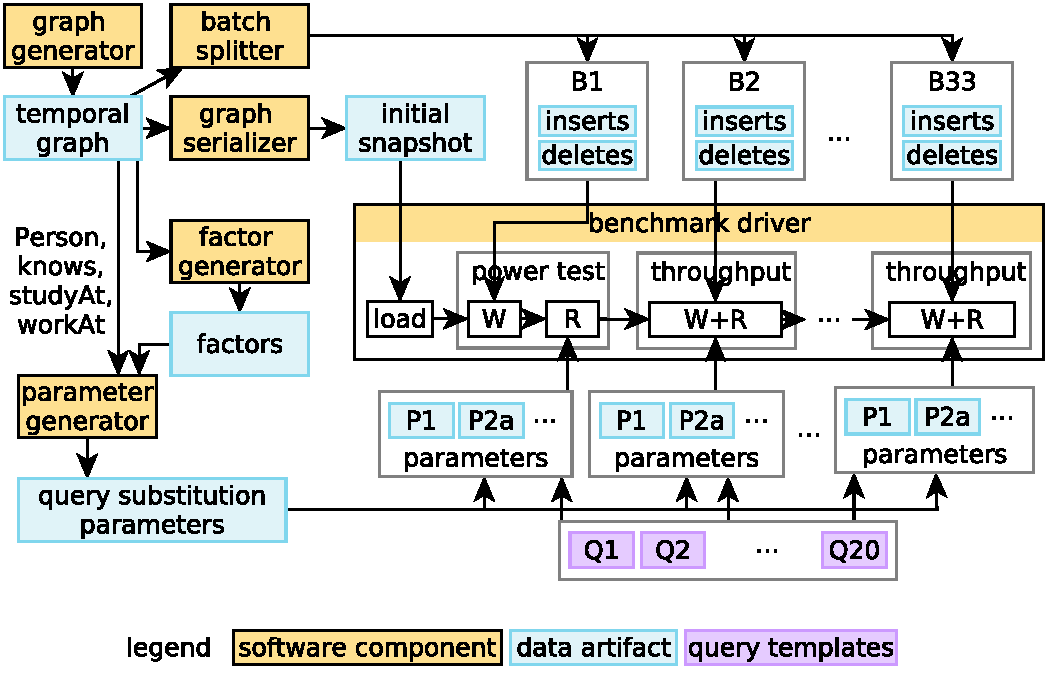
\includegraphics[scale=\yedscale]{figures/bi-workflow}
    \caption{Main software components and data artifacts of the benchmark and their connection to the workflow executed by the BI benchmark driver. Note that unlike SNB Interactive, the BI workload does not have a warmup period.}
    \label{fig:bi-workflow}
\end{figure}

The workflow of the BI workload is shown in \autoref{fig:bi-workflow}.
The read query variants (Q1, Q2a, \ldots) are executed with 30~different substitution parameters in each batch.

\section{Parameter Selection}
\label{sec:bi-paramgen}

During data generation, a sequence of \emph{substitution parameters}
\iftoggle{StandaloneWorkloadSpecification}{}{(\autoref{sec:substitution-parameters})}
is generated.
Similarly to the Interactive workload, the parameter generation of the BI workload uses \emph{parameter curation}~\cite{DBLP:conf/tpctc/GubichevB14} to ensure that the query runtimes are  predictable (to some extent).

Several queries use multiple variants with different sets of input parameters.
\Eg for \queryRefCard{bi-read-14}{BI}{14}, 14(A) uses close countries while 14(B) uses countries that are far from each other.

In principle, query parameters are selected so that the query touches on a similar amounts of data.
For queries which are only constrained by one parameter, we select ranges in the distribution where the starting node has a similar amount of neighbours.
For example, if the query looks for \tMessages with a given \tTag:
(1) the Datagen computes the frequency of \tMessages per \tTags as a factor table,
(2) for each \tTag, we compute its distance (absolute difference) from a given percentile of the distribution is selected (\eg the \tTag on the 75th percentile),
(3) we pick the $k$ parameters with the lowest distance.

\subsection*{Related Publications}

The draft BI workload was published at the \mbox{GRADES-NDA} workshop at \mbox{SIGMOD 2018}~\cite{DBLP:conf/grades/SzarnyasPAMPKEB18}.

%%%%%%%%%%%%%%%%%%%%%%%%%%%%%%%%%%%%%%%%%%%%%%%%%%%%%%%%%%%%%%%%%%%%%%%%%%%%%%
%%%%%%%%%%%%%%%%%%%%%%%%%%%%%%%%%%%%%%%%%%%%%%%%%%%%%%%%%%%%%%%%%%%%%%%%%%%%%%
%%%%%%%%%%%%%%%%%%%%%%%%%%%%%%%%%%%%%%%%%%%%%%%%%%%%%%%%%%%%%%%%%%%%%%%%%%%%%%

\section{Reads}
\label{sec:bi-reads}

\renewcommand*{\arraystretch}{1.1}

\subsection*{BI / read / 1}
\label{section:bi-read-01}

\renewcommand{\currentQueryCard}{1}
    \marginpar{
	\raggedleft
	\vspace{0.22ex}

    \queryRefCard{bi-read-01}{BI}{1}\\
    \queryRefCard{bi-read-02}{BI}{2}\\
    \queryRefCard{bi-read-03}{BI}{3}\\
    \queryRefCard{bi-read-04}{BI}{4}\\
    \queryRefCard{bi-read-05}{BI}{5}\\
    \queryRefCard{bi-read-06}{BI}{6}\\
    \queryRefCard{bi-read-07}{BI}{7}\\
    \queryRefCard{bi-read-08}{BI}{8}\\
    \queryRefCard{bi-read-09}{BI}{9}\\
    \queryRefCard{bi-read-10}{BI}{10}\\
    \queryRefCard{bi-read-11}{BI}{11}\\
    \queryRefCard{bi-read-12}{BI}{12}\\
    \queryRefCard{bi-read-13}{BI}{13}\\
    \queryRefCard{bi-read-14}{BI}{14}\\
    \queryRefCard{bi-read-15}{BI}{15}\\
    \queryRefCard{bi-read-16}{BI}{16}\\
    \queryRefCard{bi-read-17}{BI}{17}\\
    \queryRefCard{bi-read-18}{BI}{18}\\
    \queryRefCard{bi-read-19}{BI}{19}\\
    \queryRefCard{bi-read-20}{BI}{20}\\
    \queryRefCard{bi-read-21}{BI}{21}\\
    \queryRefCard{bi-read-22}{BI}{22}\\
    \queryRefCard{bi-read-23}{BI}{23}\\
    \queryRefCard{bi-read-24}{BI}{24}\\
    \queryRefCard{bi-read-25}{BI}{25}\\
}



\noindent\begin{tabularx}{\queryCardWidth}{|>{\queryPropertyCell}p{\queryPropertyCellWidth}|X|}
	\hline
	query & BI / read / 1 \\ \hline
%
	title & Posting summary
 \\ \hline
%
	pattern & \hfill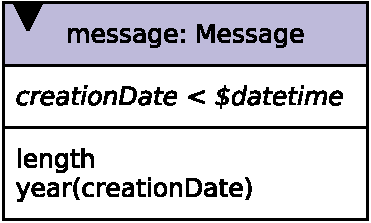
\includegraphics[scale=\patternscale,margin=0cm .2cm]{patterns/bi-read-01}\hfill\vadjust{} \\ \hline
%
	desc. & Given a date, find all \emph{Messages} created before that date. Group
them by a 3-level grouping:

\begin{enumerate}
\def\labelenumi{\arabic{enumi}.}
\tightlist
\item
  by year of creation
\item
  for each year, group into \emph{Message} types: is \emph{Comment} or
  not
\item
  for each year-type group, split into four groups based on length of
  their content

  \begin{itemize}
  \tightlist
  \item
    \texttt{0}: 0 \textless{}= length \textless{} 40~(short)
  \item
    \texttt{1}: 40 \textless{}= length \textless{} 80~(one liner)
  \item
    \texttt{2}: 80 \textless{}= length \textless{} 160~(tweet)
  \item
    \texttt{3}: 160 \textless{}= length~(long)
  \end{itemize}
\end{enumerate}
 \\ \hline
%
	
		params &
		\innerCardVSpace{\begin{tabularx}{\attributeCardWidth}{|>{\paramNumberCell}c|>{\varNameCell}M|>{\typeCell}m{\typeWidth}|Y|} \hline
		$\mathsf{1}$ & date
 & Date
 &  \\ \hline
		\end{tabularx}}\innerCardVSpace \\ \hline
	
%
	
		result &
		\innerCardVSpace{\begin{tabularx}{\attributeCardWidth}{|>{\resultNumberCell}c|>{\varNameCell}M|>{\typeCell}m{\typeWidth}|>{\resultOriginCell}c|Y|} \hline
		$\mathsf{1}$ & messageYear & 32-bit Integer & R &
				Year of the \emph{Message}
 \\ \hline
		$\mathsf{2}$ & isComment & Boolean & M &
				\texttt{true} for \emph{Comments}, \texttt{false} for \emph{Posts}
 \\ \hline
		$\mathsf{3}$ & lengthCategory & String & C &
				\texttt{0} for short, \texttt{1} for one-liner, \texttt{2} for tweet,
\texttt{3} for long
 \\ \hline
		$\mathsf{4}$ & messageCount & 32-bit Integer & A &
				Total number of \emph{Messages} in that group
 \\ \hline
		$\mathsf{5}$ & averageMessageLength & 32-bit Integer & A &
				Average length of the \emph{Message} content in that group
 \\ \hline
		$\mathsf{6}$ & sumMessageLength & 32-bit Integer & A &
				Sum of all \emph{Message} content lengths
 \\ \hline
		$\mathsf{7}$ & percentageOfMessages & 32-bit Float & A &
				Number of \emph{Messages} in group as a percentage of all messages
created before the given date
 \\ \hline
		\end{tabularx}}\innerCardVSpace \\ \hline
	
%
	
		sort		&
		\innerCardVSpace{\begin{tabularx}{\attributeCardWidth}{|>{\sortNumberCell}c|>{\varNameCell}M|>{\directionCell}c|Y|} \hline
		$\mathsf{1}$ & year
 & $\desc
$ &  \\ \hline
		$\mathsf{2}$ & isComment
 & $\asc
$ & \texttt{false\ \textless{}\ true}, i.e.~the ordering puts \emph{Posts}
first, and \emph{Comments} second
 \\ \hline
		$\mathsf{3}$ & lengthCategory
 & $\asc
$ & order based on the length of the category, \texttt{0} (short),
\texttt{1} (one liner), etc.
 \\ \hline
		\end{tabularx}}\innerCardVSpace \\ \hline
	%
	%
	CPs &
	\multicolumn{1}{>{\raggedright}l|}{
		\chokePoint{1.2}, 
		\chokePoint{3.2}, 
		\chokePoint{4.1}
		} \\ \hline
	%
	%
\end{tabularx}
\queryCardVSpace
\renewcommand*{\arraystretch}{1.1}

\subsection*{BI / read / 2}
\label{section:bi-read-02}

\renewcommand{\currentQueryCard}{2}
    \marginpar{
	\raggedleft
	\vspace{0.22ex}

    \queryRefCard{bi-read-01}{BI}{1}\\
    \queryRefCard{bi-read-02}{BI}{2}\\
    \queryRefCard{bi-read-03}{BI}{3}\\
    \queryRefCard{bi-read-04}{BI}{4}\\
    \queryRefCard{bi-read-05}{BI}{5}\\
    \queryRefCard{bi-read-06}{BI}{6}\\
    \queryRefCard{bi-read-07}{BI}{7}\\
    \queryRefCard{bi-read-08}{BI}{8}\\
    \queryRefCard{bi-read-09}{BI}{9}\\
    \queryRefCard{bi-read-10}{BI}{10}\\
    \queryRefCard{bi-read-11}{BI}{11}\\
    \queryRefCard{bi-read-12}{BI}{12}\\
    \queryRefCard{bi-read-13}{BI}{13}\\
    \queryRefCard{bi-read-14}{BI}{14}\\
    \queryRefCard{bi-read-15}{BI}{15}\\
    \queryRefCard{bi-read-16}{BI}{16}\\
    \queryRefCard{bi-read-17}{BI}{17}\\
    \queryRefCard{bi-read-18}{BI}{18}\\
    \queryRefCard{bi-read-19}{BI}{19}\\
    \queryRefCard{bi-read-20}{BI}{20}\\
    \queryRefCard{bi-read-21}{BI}{21}\\
    \queryRefCard{bi-read-22}{BI}{22}\\
    \queryRefCard{bi-read-23}{BI}{23}\\
    \queryRefCard{bi-read-24}{BI}{24}\\
    \queryRefCard{bi-read-25}{BI}{25}\\
}



\noindent\begin{tabularx}{\queryCardWidth}{|>{\queryPropertyCell}p{\queryPropertyCellWidth}|X|}
	\hline
	query & BI / read / 2 \\ \hline
%
	title & Top tags for country, age, gender, time
 \\ \hline
%
	pattern & \hfill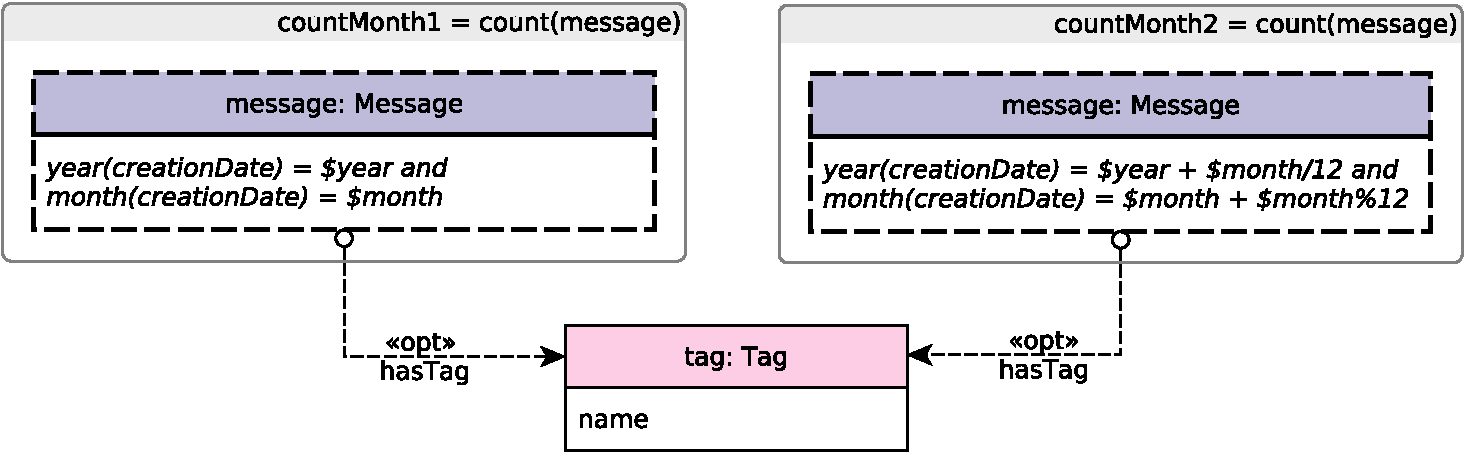
\includegraphics[scale=\patternscale,margin=0cm .2cm]{patterns/bi-read-02}\hfill\vadjust{} \\ \hline
%
	desc. & Select all \emph{Messages} created between \texttt{date1}-\texttt{date2}
(inclusive) by \emph{Persons} located in \texttt{country1} or
\texttt{country2}. Select the creator \emph{Persons} and the \emph{Tags}
of these \emph{Messages}. Split these \emph{Persons}, \emph{Tags} and
\emph{Messages} into a 5-level grouping:

\begin{enumerate}
\def\labelenumi{\arabic{enumi}.}
\tightlist
\item
  name of country of \emph{Person},
\item
  month the \emph{Message} was created,
\item
  gender of \emph{Person},
\item
  age group of \emph{Person}, defined as years between person's birthday
  and end of simulation (2013-01-01), divided by 5, rounded down,
\item
  name of tag attached to \emph{Message}.
\end{enumerate}

Consider only those groups where number of \emph{Messages} is greater
than 100.
 \\ \hline
%
	
		params &
		\innerCardVSpace{\begin{tabularx}{\attributeCardWidth}{|>{\paramNumberCell}c|>{\varNameCell}M|>{\typeCell}m{\typeWidth}|Y|} \hline
		$\mathsf{1}$ & date1
 & Date
 &  \\ \hline
		$\mathsf{2}$ & date2
 & Date
 &  \\ \hline
		$\mathsf{3}$ & country1
 & String
 &  \\ \hline
		$\mathsf{4}$ & country2
 & String
 &  \\ \hline
		\end{tabularx}}\innerCardVSpace \\ \hline
	
%
	
		result &
		\innerCardVSpace{\begin{tabularx}{\attributeCardWidth}{|>{\resultNumberCell}c|>{\varNameCell}M|>{\typeCell}m{\typeWidth}|>{\resultOriginCell}c|Y|} \hline
		$\mathsf{1}$ & country.name & String & R &
				 \\ \hline
		$\mathsf{2}$ & messageMonth & 32-bit Integer & R &
				1--12
 \\ \hline
		$\mathsf{3}$ & person.gender & String & R &
				\texttt{male}/\texttt{female}
 \\ \hline
		$\mathsf{4}$ & ageGroup & 32-bit Integer & C &
				 \\ \hline
		$\mathsf{5}$ & tag.name & String & R &
				 \\ \hline
		$\mathsf{6}$ & messageCount & 64-bit Integer & A &
				The number of messages in the group
 \\ \hline
		\end{tabularx}}\innerCardVSpace \\ \hline
	
%
	
		sort		&
		\innerCardVSpace{\begin{tabularx}{\attributeCardWidth}{|>{\sortNumberCell}c|>{\varNameCell}M|>{\directionCell}c|Y|} \hline
		$\mathsf{1}$ & messageCount
 & $\desc
$ &  \\ \hline
		$\mathsf{2}$ & tag.name
 & $\asc
$ &  \\ \hline
		$\mathsf{3}$ & ageGroup
 & $\asc
$ &  \\ \hline
		$\mathsf{4}$ & person.gender
 & $\asc
$ &  \\ \hline
		$\mathsf{5}$ & messageMonth
 & $\asc
$ &  \\ \hline
		$\mathsf{6}$ & country.name
 & $\asc
$ &  \\ \hline
		\end{tabularx}}\innerCardVSpace \\ \hline
	%
	limit & 100 \\ \hline
	%
	CPs &
	\multicolumn{1}{>{\raggedright}l|}{
		\chokePoint{1.1}, 
		\chokePoint{1.2}, 
		\chokePoint{1.4}, 
		\chokePoint{2.1}, 
		\chokePoint{2.3}, 
		\chokePoint{3.1}, 
		\chokePoint{3.2}
		} \\ \hline
	%
	%
\end{tabularx}
\queryCardVSpace
\renewcommand*{\arraystretch}{1.1}

\subsection*{BI / read / 3}
\label{section:bi-read-03}

\noindent\begin{tabularx}{\queryCardWidth}{|>{\queryPropertyCell}p{\queryPropertyCellWidth}|X|}
	\hline
	query & BI / read / 3 \\ \hline
%
	title & Tag evolution
 \\ \hline
%
	pattern & \hfill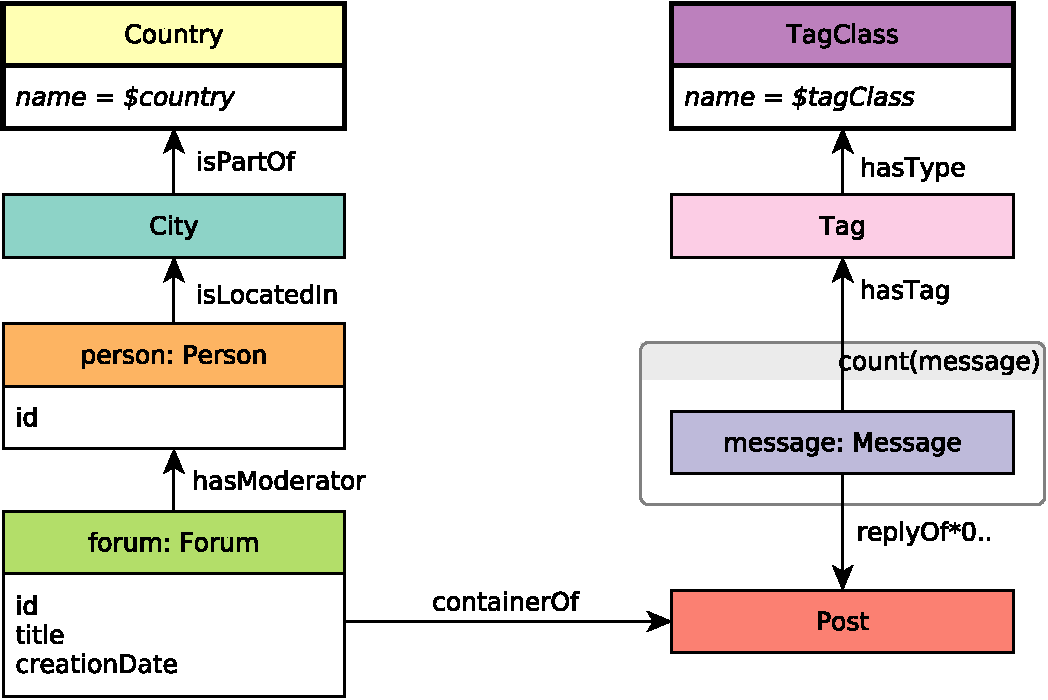
\includegraphics[scale=\patternscale,margin=0cm .2cm]{patterns/bi-read-03}\hfill\vadjust{} \\ \hline
%
	desc. & Given a year and a month, find the Tags that were used in Messages
during the given month of the given year, and the Tags that were used
during the month after the given month of the given year.

For both months, compute the count of Messages that used each of the
Tags.
 \\ \hline
%
	
		params &
		\innerCardVSpace{\begin{tabularx}{\attributeCardWidth}{|>{\paramNumberCell}c|>{\varNameCell}M|>{\typeCell}m{\typeWidth}|Y|} \hline
		$\mathsf{1}$ & year
 & 32-bit Integer
 &  \\ \hline
		$\mathsf{2}$ & month
 & 32-bit Integer
 &  \\ \hline
		\end{tabularx}}\innerCardVSpace \\ \hline
	
%
	
		result &
		\innerCardVSpace{\begin{tabularx}{\attributeCardWidth}{|>{\resultNumberCell}c|>{\varNameCell}M|>{\typeCell}m{\typeWidth}|>{\resultOriginCell}c|Y|} \hline
		$\mathsf{1}$ & tag.name
 & String
 & R &
				 \\ \hline
		$\mathsf{2}$ & countMonth1
 & 32-bit Integer
 & R &
				occurrences of the tag during year-month 1
 \\ \hline
		$\mathsf{3}$ & countMonth2
 & 32-bit Integer
 & R &
				occurrences of the tag during year-month 2
 \\ \hline
		$\mathsf{4}$ & diff
 & 32-bit Integer
 & R &
				difference between occurrences of this Tag in month 1 and month 2
 \\ \hline
		\end{tabularx}}\innerCardVSpace \\ \hline
	
%
	
		sort		&
		\innerCardVSpace{\begin{tabular}{|>{\sortNumberCell}c|>{\varNameCell}l|>{\directionCell}c|} \hline
		$\mathsf{1}$ & diff
 & $\desc
$ \\ \hline
		$\mathsf{2}$ & tag.name
 & $\asc
$ \\ \hline
		\end{tabular}}\innerCardVSpace \\ \hline
	%
	limit & 100 \\ \hline
	%
	CPs &
	\multicolumn{1}{>{\raggedright}l|}{
		\chokePoint{2.4}, 
		\chokePoint{3.1}, 
		\chokePoint{3.2}, 
		\chokePoint{4.1}, 
		\chokePoint{4.3}, 
		\chokePoint{5.3}, 
		\chokePoint{6.1}
		} \\ \hline
	%
	%
\end{tabularx}
\queryCardVSpace
\renewcommand*{\arraystretch}{1.1}

\noindent\begin{tabularx}{17cm}{|>{\small \sf}c|X|}
	\hline
	query    & BI / 4 \\ \hline
%
	title       & Popular topics in a country \\ \hline
%
    pattern     & \hfill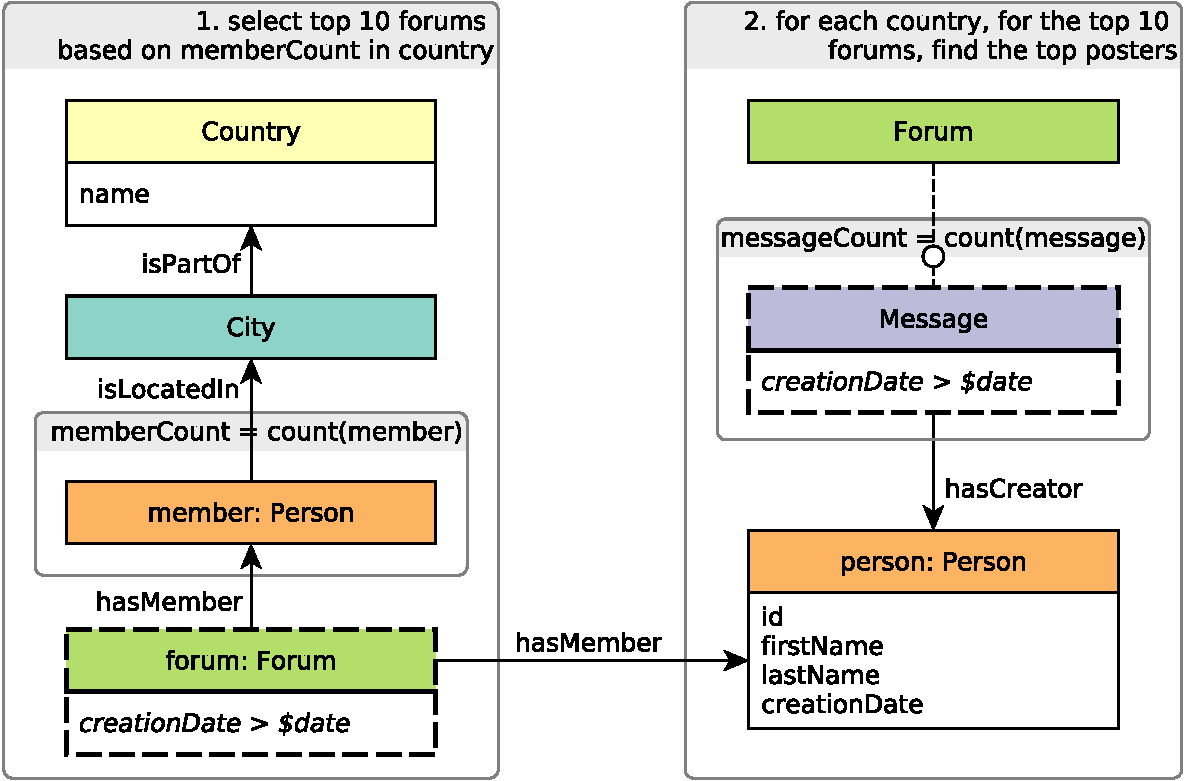
\includegraphics[scale=\patternscale,margin=0cm .2cm]{patterns/bi-read-04}\hfill\vadjust{} \\ \hline
%
	desc. & Given a TagClass and a Country, find all the Forums created in the given
Country, containing at least one Post with Tags belonging directly to
the given TagClass.

The location of a Forum is identified by the location of the Forum's
moderator.
 \\ \hline
%
	
%
	params  &
	\vspace{1.1ex}{\begin{tabularx}{14.66cm}{|c|M|m{2cm}|Y|} \hline
	\cellcolor{parameter} \color{white} \footnotesize $\mathsf{1}$ & \varname{tagClass} & \cellcolor{gray!20} \vartype{32-bit Integer} &  \\ \hline
	\cellcolor{parameter} \color{white} \footnotesize $\mathsf{2}$ & \varname{country} & \cellcolor{gray!20} \vartype{32-bit Integer} &  \\ \hline
	\end{tabularx}}\vspace{1.1ex} \\ \hline
%
	
	result      &
	\vspace{1.1ex}{\begin{tabularx}{14.66cm}{|c|M|m{2cm}|c|Y|} \hline
	\cellcolor{result} \color{white} \footnotesize $\mathsf{1}$ & \varname{forum.id} & \cellcolor{gray!20} \vartype{64-bit Integer} &
	    \texttt{R} &
	     \\ \hline
	\cellcolor{result} \color{white} \footnotesize $\mathsf{2}$ & \varname{forum.title} & \cellcolor{gray!20} \vartype{String} &
	    \texttt{R} &
	     \\ \hline
	\cellcolor{result} \color{white} \footnotesize $\mathsf{3}$ & \varname{forum.creationDate} & \cellcolor{gray!20} \vartype{DateTime} &
	    \texttt{R} &
	     \\ \hline
	\cellcolor{result} \color{white} \footnotesize $\mathsf{4}$ & \varname{person.id} & \cellcolor{gray!20} \vartype{64-bit Integer} &
	    \texttt{R} &
	     \\ \hline
	\cellcolor{result} \color{white} \footnotesize $\mathsf{5}$ & \varname{postCount} & \cellcolor{gray!20} \vartype{32-bit Integer} &
	    \texttt{A} &
	     \\ \hline
	\end{tabularx}}\vspace{1.1ex} \\ \hline
	
%
	sort        &
	\vspace{1.1ex}{\begin{tabular}{|c|l|c|} \hline
	\cellcolor{sort} \color{white} \footnotesize $\mathsf{1}$ & \varname{count} & \cellcolor{gray!20} $\desc$ \\ \hline
	\cellcolor{sort} \color{white} \footnotesize $\mathsf{2}$ & \varname{forum.id} & \cellcolor{gray!20} $\asc$ \\ \hline
	\end{tabular}}\vspace{1.1ex} \\ \hline
	%
	limit       & 20 \\ \hline
	%
	CPs &
	\multicolumn{1}{>{\raggedright}l|}{
	  \chokepoint{1.1}, 
	  \chokepoint{1.2}, 
	  \chokepoint{1.4}, 
	  \chokepoint{2.1}, 
	  \chokepoint{2.2}, 
	  \chokepoint{2.4}, 
	  \chokepoint{3.3}
	  } \\ \hline
	%
    %
\end{tabularx}
\vspace{2ex}
\renewcommand*{\arraystretch}{1.1}

\subsection*{BI / read / 5}
\label{section:bi-read-05}

% change \emph{} to use sans-serif font
\let\oldemph\emph
\renewcommand{\emph}[1]{{\footnotesize \sf #1}}

\renewcommand{\currentQueryCard}{5}
\marginpar{
	\raggedleft
	\vspace{0.22ex}

	\queryRefCard{bi-read-01}{BI}{1}\\
	\queryRefCard{bi-read-02}{BI}{2}\\
	\queryRefCard{bi-read-03}{BI}{3}\\
	\queryRefCard{bi-read-04}{BI}{4}\\
	\queryRefCard{bi-read-05}{BI}{5}\\
	\queryRefCard{bi-read-06}{BI}{6}\\
	\queryRefCard{bi-read-07}{BI}{7}\\
	\queryRefCard{bi-read-08}{BI}{8}\\
	\queryRefCard{bi-read-09}{BI}{9}\\
	\queryRefCard{bi-read-10}{BI}{10}\\
	\queryRefCard{bi-read-11}{BI}{11}\\
	\queryRefCard{bi-read-12}{BI}{12}\\
	\queryRefCard{bi-read-13}{BI}{13}\\
	\queryRefCard{bi-read-14}{BI}{14}\\
	\queryRefCard{bi-read-15}{BI}{15}\\
	\queryRefCard{bi-read-16}{BI}{16}\\
	\queryRefCard{bi-read-17}{BI}{17}\\
	\queryRefCard{bi-read-18}{BI}{18}\\
	\queryRefCard{bi-read-19}{BI}{19}\\
	\queryRefCard{bi-read-20}{BI}{20}\\
	\queryRefCard{bi-read-21}{BI}{21}\\
	\queryRefCard{bi-read-22}{BI}{22}\\
	\queryRefCard{bi-read-23}{BI}{23}\\
	\queryRefCard{bi-read-24}{BI}{24}\\
	\queryRefCard{bi-read-25}{BI}{25}\\
}



\noindent\begin{tabularx}{\queryCardWidth}{|>{\queryPropertyCell}p{\queryPropertyCellWidth}|X|}
	\hline
	query & BI / read / 5 \\ \hline
%
	title & Top posters in a country \\ \hline
%
	pattern & \multicolumn{1}{c|}{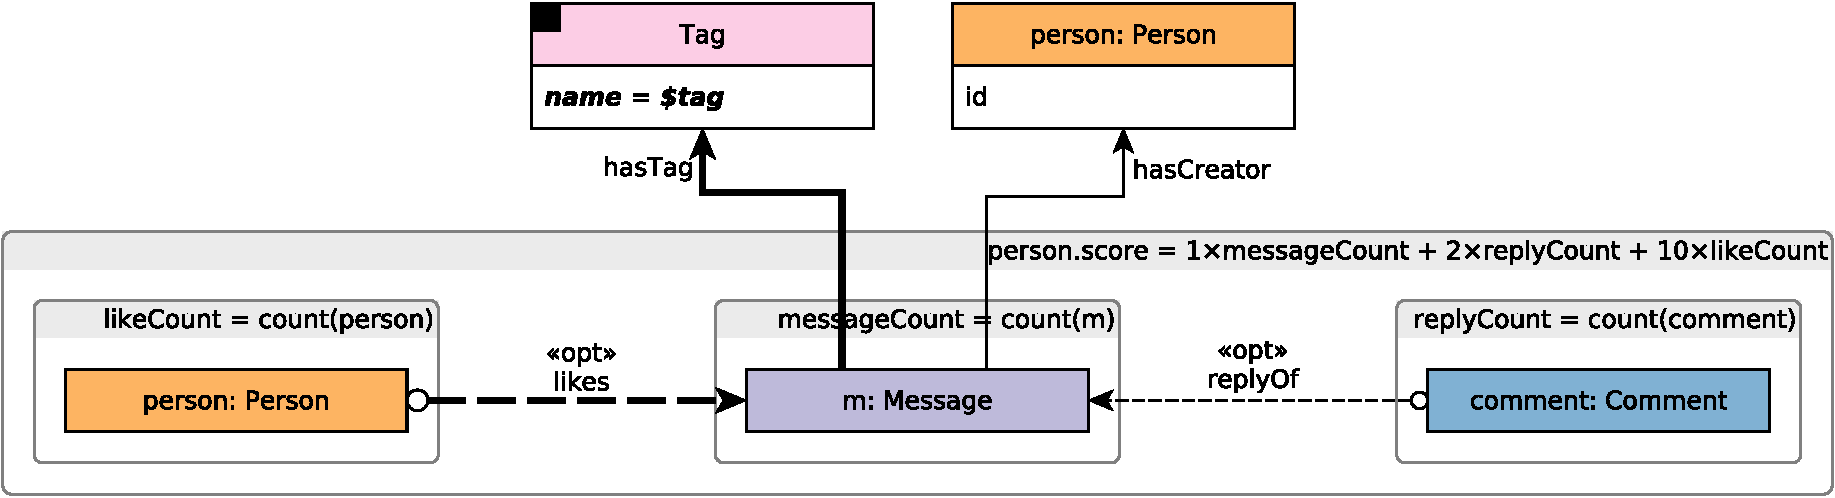
\includegraphics[scale=\patternscale,margin=0cm .2cm]{patterns/bi-read-05}} \\ \hline
%
	desc. & Find the most popular \emph{Forums} for a given \emph{Country}, where
the popularity of a \emph{Forum} is measured by the number of members
that \emph{Forum} has from the given \emph{Country}.

Calculate the top 100 most popular \emph{Forums}. In case of a tie, the
forum(s) with the smaller id value(s) should be selected.

For each member \emph{Person} of the 100 most popular \emph{Forums},
count the number of \emph{Posts} (\texttt{postCount}) they made in any
of those (most popular) \emph{Forums}. Also include those member
\emph{Persons} who have not posted any messages (have a
\texttt{postCount} of 0).
 \\ \hline
%
	
		params &
		\innerCardVSpace{\begin{tabularx}{\attributeCardWidth}{|>{\paramNumberCell}c|>{\varNameCell}M|>{\typeCell}m{\typeWidth}|Y|} \hline
		$\mathsf{1}$ & country
 & String
 &  \\ \hline
		\end{tabularx}}\innerCardVSpace \\ \hline
	
%
	
		result &
		\innerCardVSpace{\begin{tabularx}{\attributeCardWidth}{|>{\resultNumberCell}c|>{\varNameCell}M|>{\typeCell}m{\typeWidth}|>{\resultOriginCell}c|Y|} \hline
		$\mathsf{1}$ & person.id & 64-bit Integer & R &
				 \\ \hline
		$\mathsf{2}$ & person.firstName & String & R &
				 \\ \hline
		$\mathsf{3}$ & person.lastName & String & R &
				 \\ \hline
		$\mathsf{4}$ & person.creationDate & DateTime & R &
				 \\ \hline
		$\mathsf{5}$ & postCount & 32-bit Integer & A &
				 \\ \hline
		\end{tabularx}}\innerCardVSpace \\ \hline
	
%
	
		sort		&
		\innerCardVSpace{\begin{tabularx}{\attributeCardWidth}{|>{\sortNumberCell}c|>{\varNameCell}M|>{\directionCell}c|Y|} \hline
		$\mathsf{1}$ & postCount
 & $\desc
$ &  \\ \hline
		$\mathsf{2}$ & person.id
 & $\asc
$ &  \\ \hline
		\end{tabularx}}\innerCardVSpace \\ \hline
	%
	limit & 100 \\ \hline
	%
	CPs &
	\multicolumn{1}{>{\raggedright}l|}{
		\chokePoint{1.2}, 
		\chokePoint{1.3}, 
		\chokePoint{2.1}, 
		\chokePoint{2.2}, 
		\chokePoint{2.3}, 
		\chokePoint{2.4}, 
		\chokePoint{3.3}, 
		\chokePoint{5.3}, 
		\chokePoint{6.1}, 
		\chokePoint{8.2}, 
		\chokePoint{8.4}
		} \\ \hline
	%
	%
\end{tabularx}
\queryCardVSpace

% change \emph back to the old one
\let\emph\oldemph
\renewcommand*{\arraystretch}{1.1}

\subsection*{BI / read / 6}
\label{sec:bi-read-06}

\noindent\begin{tabularx}{\queryCardWidth}{|>{\queryPropertyCell}p{\queryPropertyCellWidth}|X|}
	\hline
	query & BI / read / 6 \\ \hline
%
	title & Most active Posters of a given Topic
 \\ \hline
%
	pattern & \hfill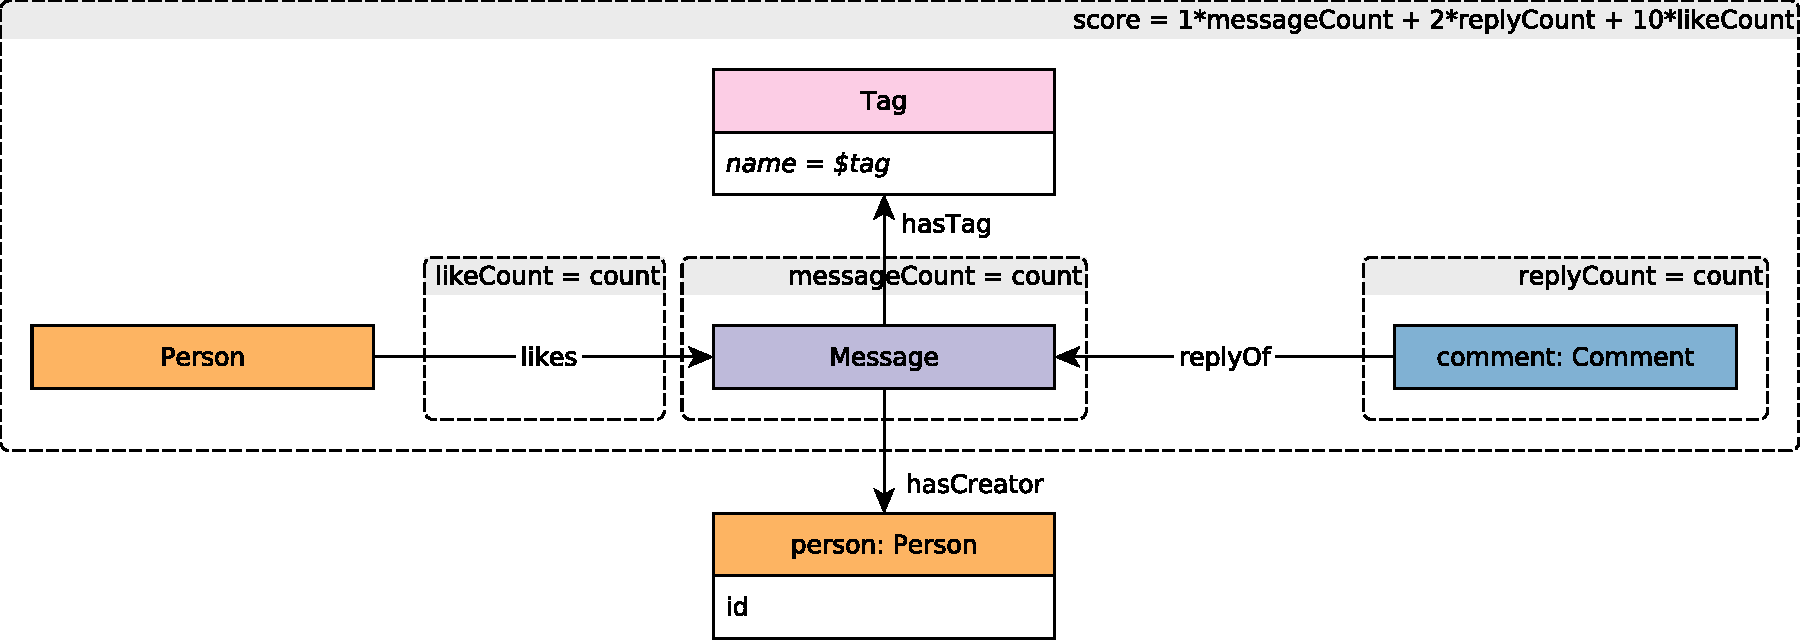
\includegraphics[scale=\patternscale,margin=0cm .2cm]{patterns/bi-read-06}\hfill\vadjust{} \\ \hline
%
	desc. & Get Persons who have created a Message (Post or Comment) with a given
Tag.

Each Person has a score, computed as follows:

\begin{itemize}
\tightlist
\item
  Count of Messages with the given Tag (\texttt{messageCount}).
\item
  Count of Likes (\texttt{likeCount}) and Comments (\texttt{replyCount})
  in reply of their Messages with the given Tag (direct relation not
  transitive).
\end{itemize}

The \texttt{score} is calculated as a sum with the following weights:

\begin{itemize}
\tightlist
\item
  Messages (\texttt{messageCount}) are multiplied by 1,
\item
  Comments to Messages (\texttt{replyCount}) are multiplied by 2,
\item
  Likes (\texttt{likeCount}) are multiplied by 10.
\end{itemize}
 \\ \hline
%
	
%
	
		params &
		\innerCardVSpace{\begin{tabularx}{\attributeCardWidth}{|>{\paramNumberCell}c|>{\varNameCell}M|>{\typeCell}m{\typeWidth}|Y|} \hline
		$\mathsf{1}$ & tag
 & 32-bit Integer
 &  \\ \hline
		\end{tabularx}}\innerCardVSpace \\ \hline
	
%
	
		result &
		\innerCardVSpace{\begin{tabularx}{\attributeCardWidth}{|>{\resultNumberCell}c|>{\varNameCell}M|>{\typeCell}m{\typeWidth}|>{\resultOriginCell}c|Y|} \hline
		$\mathsf{1}$ & person.id
 & 64-bit Integer
 & R &
				 \\ \hline
		$\mathsf{2}$ & replyCount
 & 32-bit Integer
 & R &
				 \\ \hline
		$\mathsf{3}$ & likeCount
 & 32-bit Integer
 & R &
				 \\ \hline
		$\mathsf{4}$ & messageCount
 & 32-bit Integer
 & R &
				 \\ \hline
		$\mathsf{5}$ & score
 & 32-bit Integer
 & R &
				 \\ \hline
		\end{tabularx}}\innerCardVSpace \\ \hline
	
%
	
		sort		&
		\innerCardVSpace{\begin{tabular}{|>{\sortNumberCell}c|>{\varNameCell}l|>{\directionCell}c|} \hline
		$\mathsf{1}$ & score
 & $\desc
$ \\ \hline
		$\mathsf{2}$ & person.id
 & $\asc
$ \\ \hline
		\end{tabular}}\innerCardVSpace \\ \hline
	%
	limit & 100 \\ \hline
	%
	CPs &
	\multicolumn{1}{>{\raggedright}l|}{
		\chokePoint{1.2}, 
		\chokePoint{2.3}
		} \\ \hline
	%
	%
\end{tabularx}
\queryCardVSpace
\renewcommand*{\arraystretch}{1.1}

\subsection*{BI / read / 7}
\label{section:bi-read-07}

% change \emph{} to use sans-serif font
\let\oldemph\emph
\renewcommand{\emph}[1]{{\footnotesize \sf #1}}

\renewcommand{\currentQueryCard}{7}
\marginpar{
	\raggedleft
	\vspace{0.22ex}

	\queryRefCard{bi-read-01}{BI}{1}\\
	\queryRefCard{bi-read-02}{BI}{2}\\
	\queryRefCard{bi-read-03}{BI}{3}\\
	\queryRefCard{bi-read-04}{BI}{4}\\
	\queryRefCard{bi-read-05}{BI}{5}\\
	\queryRefCard{bi-read-06}{BI}{6}\\
	\queryRefCard{bi-read-07}{BI}{7}\\
	\queryRefCard{bi-read-08}{BI}{8}\\
	\queryRefCard{bi-read-09}{BI}{9}\\
	\queryRefCard{bi-read-10}{BI}{10}\\
	\queryRefCard{bi-read-11}{BI}{11}\\
	\queryRefCard{bi-read-12}{BI}{12}\\
	\queryRefCard{bi-read-13}{BI}{13}\\
	\queryRefCard{bi-read-14}{BI}{14}\\
	\queryRefCard{bi-read-15}{BI}{15}\\
	\queryRefCard{bi-read-16}{BI}{16}\\
	\queryRefCard{bi-read-17}{BI}{17}\\
	\queryRefCard{bi-read-18}{BI}{18}\\
	\queryRefCard{bi-read-19}{BI}{19}\\
	\queryRefCard{bi-read-20}{BI}{20}\\
	\queryRefCard{bi-read-21}{BI}{21}\\
	\queryRefCard{bi-read-22}{BI}{22}\\
	\queryRefCard{bi-read-23}{BI}{23}\\
	\queryRefCard{bi-read-24}{BI}{24}\\
	\queryRefCard{bi-read-25}{BI}{25}\\
}


\noindent\begin{tabularx}{\queryCardWidth}{|>{\queryPropertyCell}p{\queryPropertyCellWidth}|X|}
	\hline
	query & BI / read / 7 \\ \hline
%
	title & Most authoritative users on a given topic \\ \hline
%
	pattern & \hfill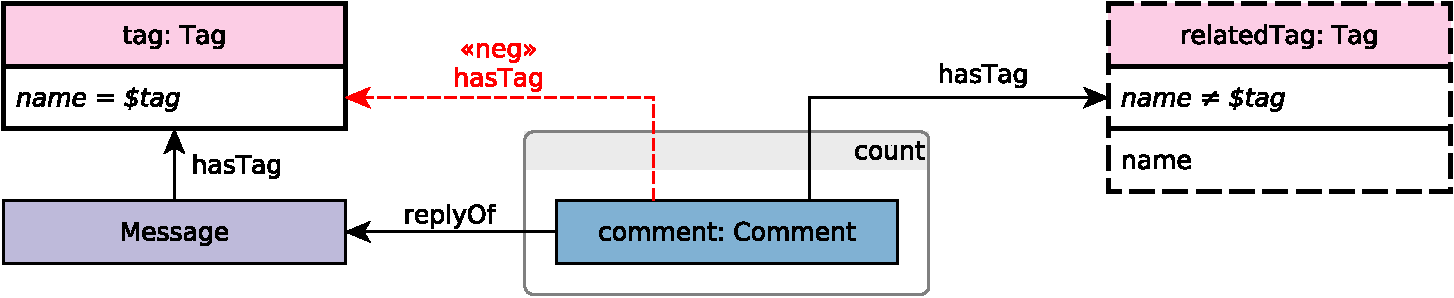
\includegraphics[scale=\patternscale,margin=0cm .2cm]{patterns/bi-read-07}\hfill\vadjust{} \\ \hline
%
	desc. & Given a \emph{Tag}, find all \emph{Persons} (\texttt{person1}) that ever
created a \emph{Message} (\texttt{message1}) with the given \emph{Tag}.
For each of these \emph{Persons} (\texttt{person}) compute their
``authority score'' as follows:

\begin{itemize}
\tightlist
\item
  The ``authority score'' is the sum of ``popularity scores'' of the
  \emph{Persons} (\texttt{person2}) that liked any of that
  \emph{Person}'s \emph{Messages} (\texttt{message2}) with the given
  \emph{Tag}.
\item
  A \emph{Person}'s (\texttt{person2}) ``popularity score'' is defined
  as the total number of likes on all of their \emph{Messages}
  (\texttt{message3}).
\end{itemize}
 \\ \hline
%
	
		params &
		\innerCardVSpace{\begin{tabularx}{\attributeCardWidth}{|>{\paramNumberCell}c|>{\varNameCell}M|>{\typeCell}m{\typeWidth}|Y|} \hline
		$\mathsf{1}$ & tag
 & String
 &  \\ \hline
		\end{tabularx}}\innerCardVSpace \\ \hline
	
%
	
		result &
		\innerCardVSpace{\begin{tabularx}{\attributeCardWidth}{|>{\resultNumberCell}c|>{\varNameCell}M|>{\typeCell}m{\typeWidth}|>{\resultOriginCell}c|Y|} \hline
		$\mathsf{1}$ & person1.id & 64-bit Integer & R &
				 \\ \hline
		$\mathsf{2}$ & authorityScore & 32-bit Integer & A &
				 \\ \hline
		\end{tabularx}}\innerCardVSpace \\ \hline
	
%
	
		sort		&
		\innerCardVSpace{\begin{tabularx}{\attributeCardWidth}{|>{\sortNumberCell}c|>{\varNameCell}M|>{\directionCell}c|Y|} \hline
		$\mathsf{1}$ & authorityScore
 & $\desc
$ &  \\ \hline
		$\mathsf{2}$ & person1.id
 & $\asc
$ &  \\ \hline
		\end{tabularx}}\innerCardVSpace \\ \hline
	%
	limit & 100 \\ \hline
	%
	CPs &
	\multicolumn{1}{>{\raggedright}l|}{
		\chokePoint{1.2}, 
		\chokePoint{2.3}, 
		\chokePoint{3.2}, 
		\chokePoint{3.3}, 
		\chokePoint{6.1}
		} \\ \hline
	%
	%
\end{tabularx}
\queryCardVSpace

% change \emph back to the old one
\renewcommand{\emph}[1]{\oldemph{#1}}
\renewcommand*{\arraystretch}{1.1}

\noindent\begin{tabularx}{17cm}{|>{\small \sf}c|X|}
	\hline
	query    & BI / 8 \\ \hline
%
	title       & Related topics \\ \hline
%
    pattern     & \hfill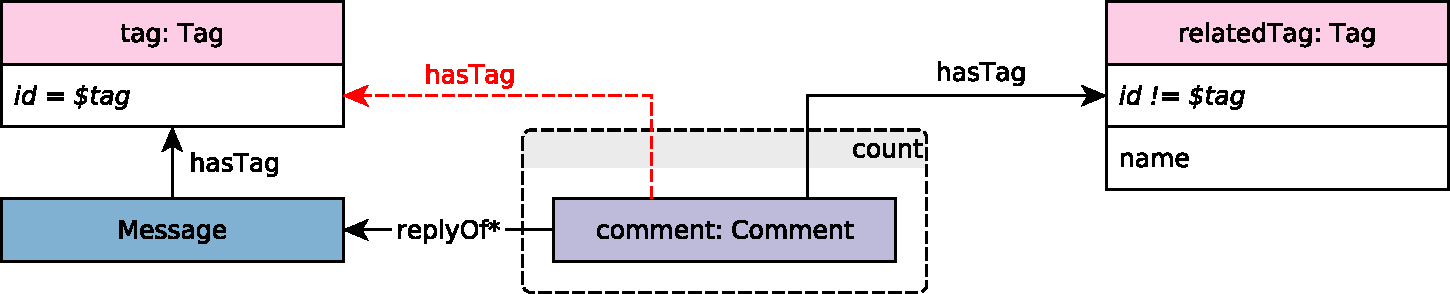
\includegraphics[scale=\patternscale,margin=0cm .2cm]{patterns/bi-read-08}\hfill\vadjust{} \\ \hline
%
	desc. & Find all Messages that have a given Tag. Find the related Tags attached
to replies of these Messages (TODO - transitive? szarnyasg), but only of
those replies that do not have the given Tag.

Group the Tags by name, and get the count of replies in each group.
 \\ \hline
%
	
	group by       &
	\multicolumn{1}{>{\raggedright}X|}{
		\varname{relatedTag.name}
		} \\ \hline
	
%
	params  &
	\vspace{1.1ex}{\begin{tabularx}{14.66cm}{|c|M|m{2cm}|Y|} \hline
	\cellcolor{parameter} \color{white} \footnotesize $\mathsf{1}$ & \varname{tag} & \cellcolor{gray!20} \vartype{32-bit Integer} &  \\ \hline
	\end{tabularx}}\vspace{1.1ex} \\ \hline
%
	
	result      &
	\vspace{1.1ex}{\begin{tabularx}{14.66cm}{|c|M|m{2cm}|c|Y|} \hline
	\cellcolor{result} \color{white} \footnotesize $\mathsf{1}$ & \varname{relatedTag.name} & \cellcolor{gray!20} \vartype{String} &
	    \texttt{R} &
	     \\ \hline
	\cellcolor{result} \color{white} \footnotesize $\mathsf{2}$ & \varname{count} & \cellcolor{gray!20} \vartype{32-bit Integer} &
	    \texttt{A} &
	     \\ \hline
	\end{tabularx}}\vspace{1.1ex} \\ \hline
	
%
	sort        &
	\vspace{1.1ex}{\begin{tabular}{|c|l|c|} \hline
	\cellcolor{sort} \color{white} \footnotesize $\mathsf{1}$ & \varname{count} & \cellcolor{gray!20} $\desc$ \\ \hline
	\cellcolor{sort} \color{white} \footnotesize $\mathsf{2}$ & \varname{relatedTag.name} & \cellcolor{gray!20} $\asc$ \\ \hline
	\end{tabular}}\vspace{1.1ex} \\ \hline
	%
	limit       & 100 \\ \hline
	%
	CPs &
	\multicolumn{1}{>{\raggedright}l|}{
	  \chokepoint{1.6}, 
	  \chokepoint{3.3}, 
	  \chokepoint{5.2}
	  } \\ \hline
	%
    %
\end{tabularx}
\vspace{2ex}
\renewcommand*{\arraystretch}{1.1}

\label{sec:bi-read-09}
\noindent\begin{tabularx}{\queryCardWidth}{|>{\queryPropertyCell}c|X|}
	\hline
	query & BI / 9 \\ \hline
%
	title & Forum with related Tags \\ \hline
%
    pattern & \hfill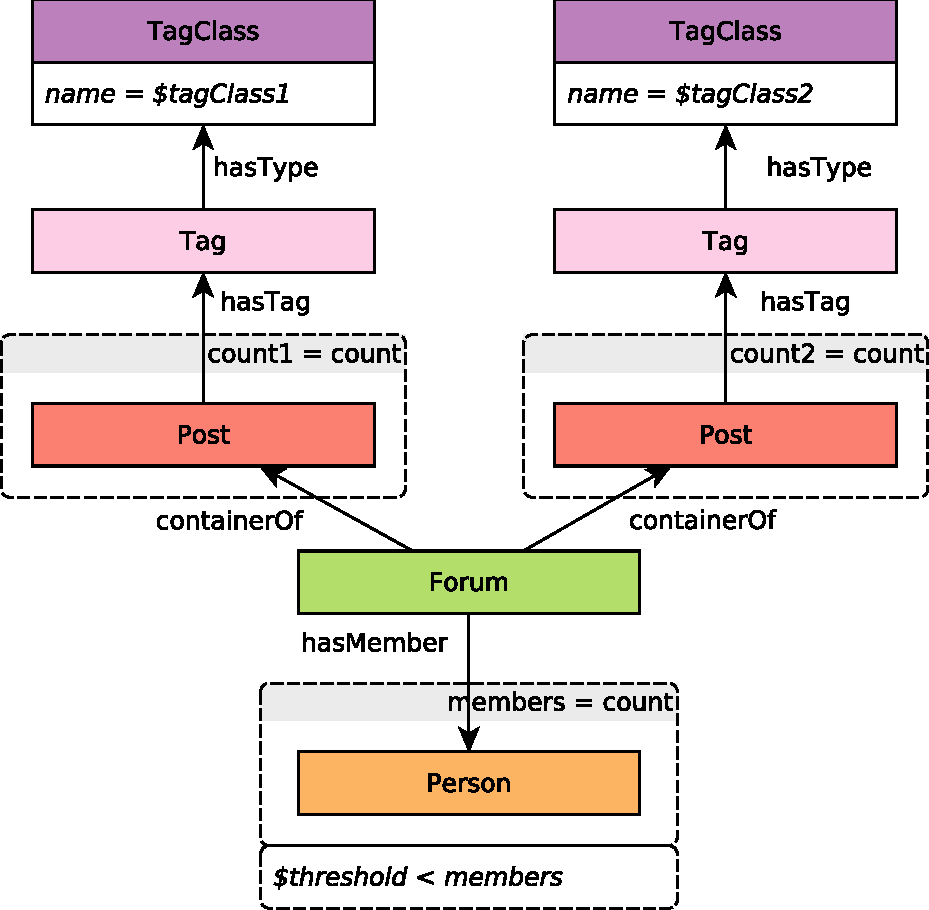
\includegraphics[scale=\patternscale,margin=0cm .2cm]{patterns/bi-read-09}\hfill\vadjust{} \\ \hline
%
	desc. & Given two TagClasses (\texttt{tagClass1} \& \texttt{tagClass2}), find
Forums that contain at least one Post with a Tag from \texttt{tagClass1}
and at least one Post with a Tag from \texttt{tagClass2} (direct
children not transitive) -- this may be the same Post.

Consider the Forums with a number of members greater than a given
threshold. For every such forum, count the number of Posts that have a
Tag from TagClass1 (count1), and the number of posts that have a tag
from TagClass2.
 \\ \hline
%
	
%
	params &
	\innerCardVSpace{\begin{tabularx}{\attributeCardWidth}{|>{\paramNumberCell}c|>{\varNameCell}M|>{\typeCell}m{\typeWidth}|Y|} \hline
	\cellcolor{parameter} \color{white} \footnotesize $\mathsf{1}$ &tagClass1& 32-bit Integer &  \\ \hline
	\cellcolor{parameter} \color{white} \footnotesize $\mathsf{2}$ &tagClass2& 32-bit Integer &  \\ \hline
	\cellcolor{parameter} \color{white} \footnotesize $\mathsf{3}$ &threshold& 32-bit Integer &  \\ \hline
	\end{tabularx}}\innerCardVSpace \\ \hline
%
	
        result &
        \innerCardVSpace{\begin{tabularx}{\attributeCardWidth}{|>{\resultNumberCell}c|>{\varNameCell}M|>{\typeCell}m{\typeWidth}|>{\resultOriginCell}c|Y|} \hline
        $\mathsf{1}$ & forum.id & 64-bit Integer &R&
                 \\ \hline
        $\mathsf{2}$ & count1 & 32-bit Integer &A&
                Number of Posts with at least one tag belonging to tagClass1 \\ \hline
        $\mathsf{3}$ & count2 & 32-bit Integer &A&
                Number of Posts with at least one tag belonging to tagClass2 \\ \hline
        \end{tabularx}}\innerCardVSpace \\ \hline
	
%
	sort        &
        \innerCardVSpace{\begin{tabular}{|>{\sortNumberCell}c|>{\varNameCell}l|>{\directionCell}c|} \hline
        $\mathsf{1}$ & count2 & $\desc$ \\ \hline
        $\mathsf{2}$ & count1 & $\desc$ \\ \hline
        $\mathsf{3}$ & forum.id & $\asc$ \\ \hline
        \end{tabular}}\innerCardVSpace \\ \hline
	%
	limit & 100 \\ \hline
	%
	CPs &
	\multicolumn{1}{>{\raggedright}l|}{
	    \chokePoint{1.2}, 
	    \chokePoint{1.4}, 
	    \chokePoint{2.1}, 
	    \chokePoint{2.3}, 
	    \chokePoint{2.4}
	    } \\ \hline
	%
    %
\end{tabularx}
\queryCardVSpace
\renewcommand*{\arraystretch}{1.1}

\subsection*{BI / read / 10}
\label{sec:bi-read-10}

\noindent\begin{tabularx}{\queryCardWidth}{|>{\queryPropertyCell}p{\queryPropertyCellWidth}|X|}
	\hline
	query & BI / read / 10 \\ \hline
%
	title & Central Person for a Tag \\ \hline
%
	pattern & \hfill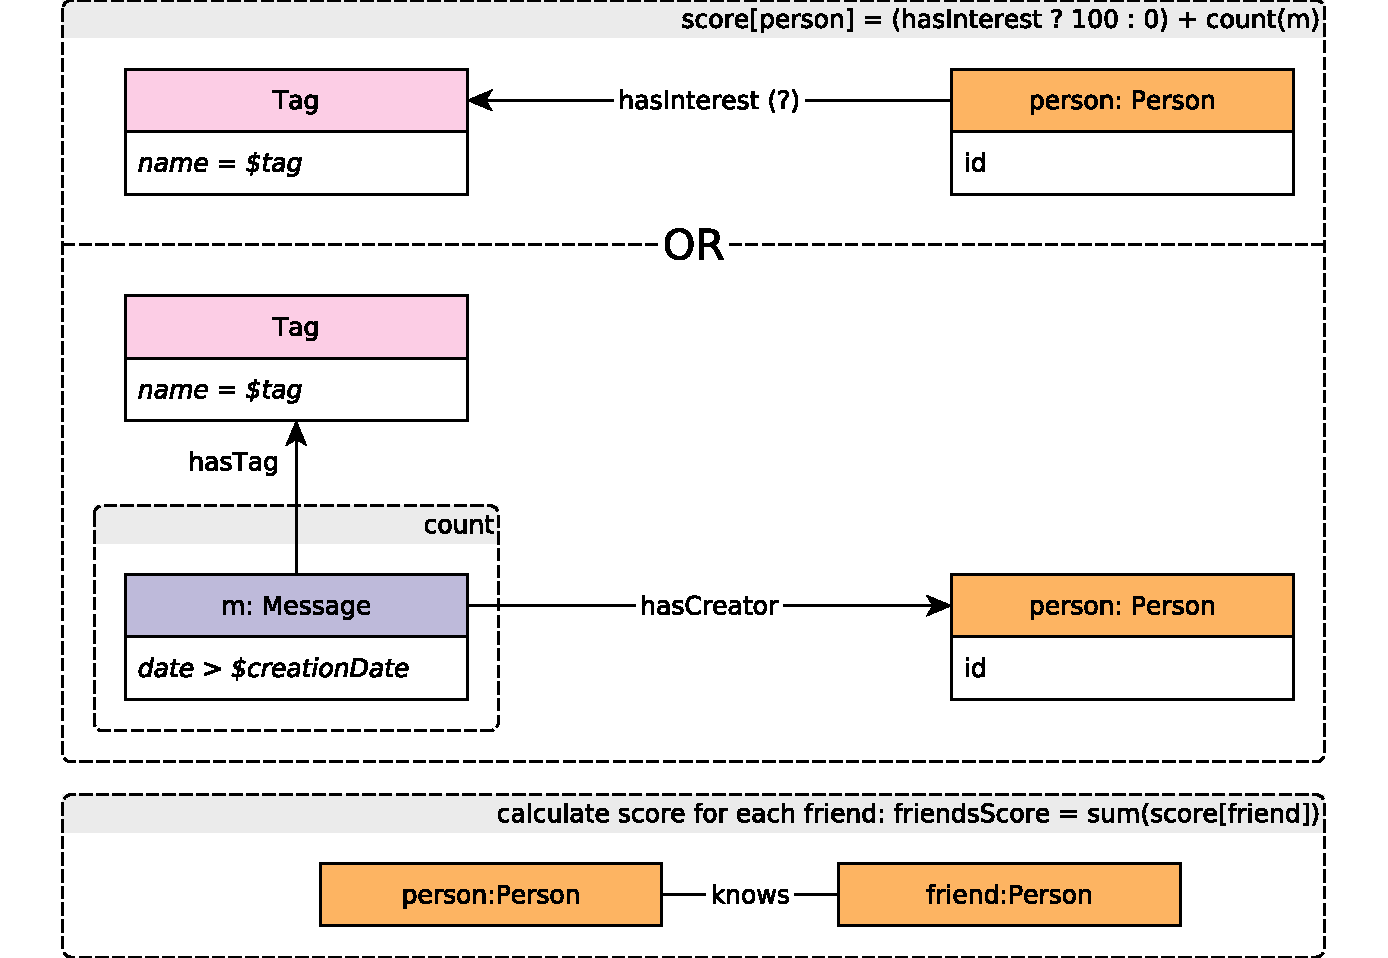
\includegraphics[scale=\patternscale,margin=0cm .2cm]{patterns/bi-read-10}\hfill\vadjust{} \\ \hline
%
	desc. & Given a Tag, find all Persons that are either interested in the Tag, or
have written a Message (Post or Comment) with creation date after a
given date and that has a given Tag. For each Person, compute the score
as the sum of the following two aspects:

\begin{itemize}
\tightlist
\item
  100, if the Person has this tag as their interest, or 0 otherwise
\item
  number of messages by this person with the given tag
\end{itemize}
 \\ \hline
%
	
%
	
		params &
		\innerCardVSpace{\begin{tabularx}{\attributeCardWidth}{|>{\paramNumberCell}c|>{\varNameCell}M|>{\typeCell}m{\typeWidth}|Y|} \hline
		$\mathsf{1}$ & tag & 32-bit Integer &  \\ \hline
		$\mathsf{2}$ & date & Date &  \\ \hline
		\end{tabularx}}\innerCardVSpace \\ \hline
	
%
	
		result &
		\innerCardVSpace{\begin{tabularx}{\attributeCardWidth}{|>{\resultNumberCell}c|>{\varNameCell}M|>{\typeCell}m{\typeWidth}|>{\resultOriginCell}c|Y|} \hline
		$\mathsf{1}$ & person.id & 64-bit Integer &R&
				 \\ \hline
		$\mathsf{2}$ & score & 32-bit Integer &A&
				 \\ \hline
		$\mathsf{3}$ & friendsScore & 32-bit Integer &A&
				The sum of the score of the Person's friends \\ \hline
		\end{tabularx}}\innerCardVSpace \\ \hline
	
%
	sort		&
		\innerCardVSpace{\begin{tabular}{|>{\sortNumberCell}c|>{\varNameCell}l|>{\directionCell}c|} \hline
		$\mathsf{1}$ & score + friendsScore & $\desc$ \\ \hline
		$\mathsf{2}$ & person.id & $\asc$ \\ \hline
		\end{tabular}}\innerCardVSpace \\ \hline
	%
	limit & 100 \\ \hline
	%
	CPs &
	\multicolumn{1}{>{\raggedright}l|}{
		\chokePoint{1.2}, 
		\chokePoint{2.1}, 
		\chokePoint{2.3}, 
		\chokePoint{3.2}
		} \\ \hline
	%
	%
\end{tabularx}
\queryCardVSpace
\renewcommand*{\arraystretch}{1.1}

\noindent\begin{tabularx}{17cm}{|>{\small \sf}c|X|}
	\hline
	query    & BI / 11 \\ \hline
%
	title       & Unrelated replies \\ \hline
%
    pattern     & \hfill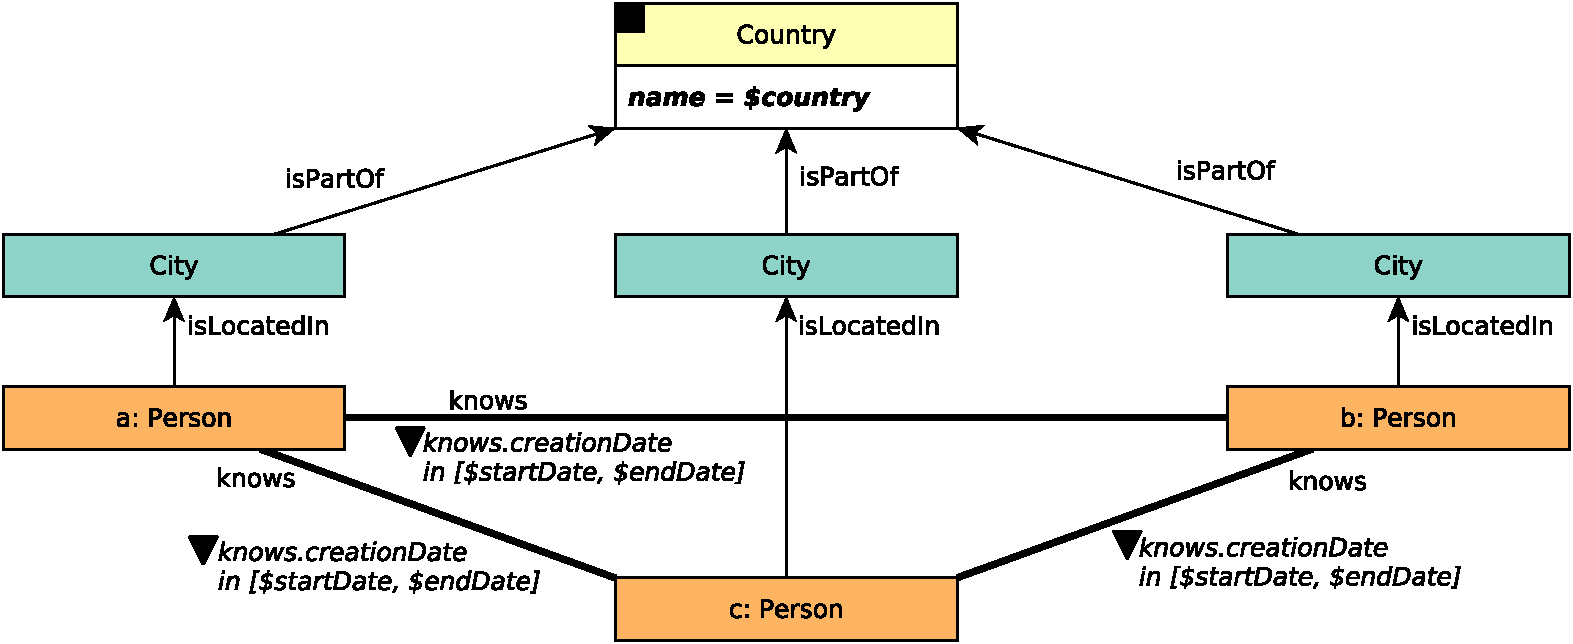
\includegraphics[scale=\patternscale,margin=0cm .2cm]{patterns/bi-read-11}\hfill\vadjust{} \\ \hline
%
	desc. & Find those Persons of a given country that replied to any Message, such
that the reply does not have any Tag in common with the Message {[}are
transitive replies considered or not? - SzG{]}. Consider only those
replies not containing any word from a given blacklist. For each Person
and valid reply, retrieve the Tags associated with the reply, and
retrieve the number of likes on the reply.
 \\ \hline
%
	
	group by       &
	\multicolumn{1}{>{\raggedright}X|}{
		\varname{person.id}, 
		\varname{tag.name}
		} \\ \hline
	
%
	params.  &
	\vspace{1.1ex}{\begin{tabularx}{14.66cm}{|c|M|m{2cm}|Y|} \hline
	\cellcolor{parameter} \color{white} $\mathsf{1}$ & \varname{country} & \cellcolor{gray!20} \vartype{32-bit Integer} &  \\ \hline
	\cellcolor{parameter} \color{white} $\mathsf{2}$ & \varname{blacklist} & \cellcolor{gray!20} \vartype{String[]} &  \\ \hline
	\end{tabularx}}\vspace{1.1ex} \\ \hline
%
	
	result      &
	\vspace{1.1ex}{\begin{tabularx}{14.66cm}{|c|M|m{2cm}|c|Y|} \hline
	\cellcolor{result} \color{white} $\mathsf{1}$ & \varname{person.id} & \cellcolor{gray!20} \vartype{64-bit Integer} &
	    \texttt{R} &
	     \\ \hline
	\cellcolor{result} \color{white} $\mathsf{2}$ & \varname{tag.name} & \cellcolor{gray!20} \vartype{String} &
	    \texttt{R} &
	     \\ \hline
	\cellcolor{result} \color{white} $\mathsf{3}$ & \varname{countLikes} & \cellcolor{gray!20} \vartype{32-bit Integer} &
	    \texttt{A} &
	    The count of Likes to replies with that Tag. \\ \hline
	\cellcolor{result} \color{white} $\mathsf{4}$ & \varname{countReplies} & \cellcolor{gray!20} \vartype{32-bit Integer} &
	    \texttt{A} &
	    The count of replies with that Tag. \\ \hline
	\end{tabularx}}\vspace{1.1ex} \\ \hline
	
%
	sort        &
	\vspace{1.1ex}{\begin{tabular}{|c|l|c|} \hline
	\cellcolor{sort} \color{white} $\mathsf{1}$ & \varname{countLikes} & \cellcolor{gray!20} $\desc$ \\ \hline
	\cellcolor{sort} \color{white} $\mathsf{2}$ & \varname{person.id} & \cellcolor{gray!20} $\asc$ \\ \hline
	\cellcolor{sort} \color{white} $\mathsf{3}$ & \varname{tag.name} & \cellcolor{gray!20} $\asc$ \\ \hline
	\end{tabular}}\vspace{1.1ex} \\ \hline
	%
	limit       & 100 \\ \hline
	%
	CPs &
	\multicolumn{1}{>{\raggedright}l|}{
	  \chokepoint{1.1}, 
	  \chokepoint{2.1}, 
	  \chokepoint{2.2}, 
	  \chokepoint{2.3}, 
	  \chokepoint{3.1}, 
	  \chokepoint{3.2}, 
	  \chokepoint{6.1}
	  } \\ \hline
	%
    %
\end{tabularx}
\vspace{2ex}
\renewcommand*{\arraystretch}{1.1}

\subsection*{BI / read / 12}
\label{section:bi-read-12}

% change \emph{} to use sans-serif font
\let\oldemph\emph
\renewcommand{\emph}[1]{{\footnotesize \sf #1}}

\renewcommand{\currentQueryCard}{12}
\marginpar{
	\raggedleft
	\vspace{0.22ex}

    \queryRefCard{bi-read-01}{BI}{1}\\
    \queryRefCard{bi-read-02}{BI}{2}\\
    \queryRefCard{bi-read-03}{BI}{3}\\
    \queryRefCard{bi-read-04}{BI}{4}\\
    \queryRefCard{bi-read-05}{BI}{5}\\
    \queryRefCard{bi-read-06}{BI}{6}\\
    \queryRefCard{bi-read-07}{BI}{7}\\
    \queryRefCard{bi-read-08}{BI}{8}\\
    \queryRefCard{bi-read-09}{BI}{9}\\
    \queryRefCard{bi-read-10}{BI}{10}\\
    \queryRefCard{bi-read-11}{BI}{11}\\
    \queryRefCard{bi-read-12}{BI}{12}\\
    \queryRefCard{bi-read-13}{BI}{13}\\
    \queryRefCard{bi-read-14}{BI}{14}\\
    \queryRefCard{bi-read-15}{BI}{15}\\
    \queryRefCard{bi-read-16}{BI}{16}\\
    \queryRefCard{bi-read-17}{BI}{17}\\
    \queryRefCard{bi-read-18}{BI}{18}\\
    \queryRefCard{bi-read-19}{BI}{19}\\
    \queryRefCard{bi-read-20}{BI}{20}\\
    \queryRefCard{bi-read-21}{BI}{21}\\
    \queryRefCard{bi-read-22}{BI}{22}\\
    \queryRefCard{bi-read-23}{BI}{23}\\
    \queryRefCard{bi-read-24}{BI}{24}\\
    \queryRefCard{bi-read-25}{BI}{25}\\
}



\noindent\begin{tabularx}{\queryCardWidth}{|>{\queryPropertyCell}p{\queryPropertyCellWidth}|X|}
	\hline
	query & BI / read / 12 \\ \hline
%
	title & Trending Posts
 \\ \hline
%
	pattern & \hfill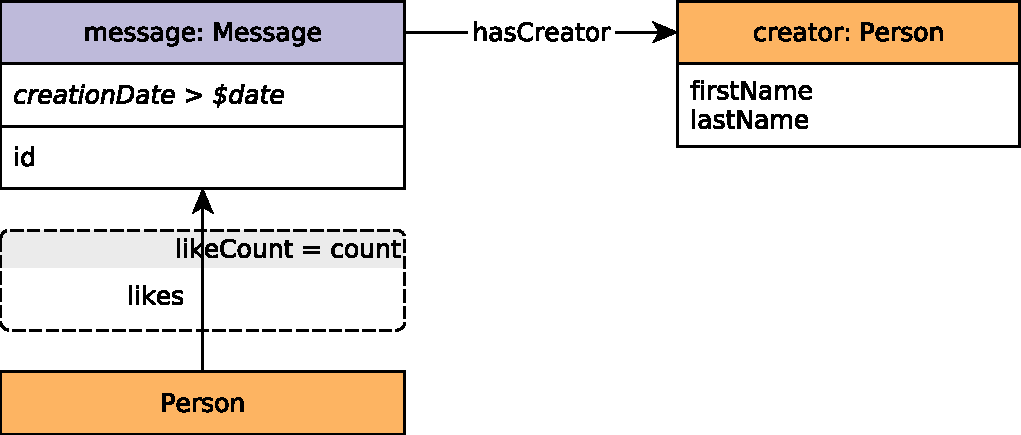
\includegraphics[scale=\patternscale,margin=0cm .2cm]{patterns/bi-read-12}\hfill\vadjust{} \\ \hline
%
	desc. & Find all \emph{Messages} created after a given \texttt{date}
(exclusive), that received more than a given number of likes
(\texttt{likeThreshold}).
 \\ \hline
%
	
		params &
		\innerCardVSpace{\begin{tabularx}{\attributeCardWidth}{|>{\paramNumberCell}c|>{\varNameCell}M|>{\typeCell}m{\typeWidth}|Y|} \hline
		$\mathsf{1}$ & date
 & Date
 &  \\ \hline
		$\mathsf{2}$ & likeThreshold
 & 32-bit Integer
 &  \\ \hline
		\end{tabularx}}\innerCardVSpace \\ \hline
	
%
	
		result &
		\innerCardVSpace{\begin{tabularx}{\attributeCardWidth}{|>{\resultNumberCell}c|>{\varNameCell}M|>{\typeCell}m{\typeWidth}|>{\resultOriginCell}c|Y|} \hline
		$\mathsf{1}$ & message.id & 64-bit Integer & R &
				 \\ \hline
		$\mathsf{2}$ & message.creationDate & DateTime & R &
				 \\ \hline
		$\mathsf{3}$ & creator.firstName & String & R &
				The first name of the \emph{Post}'s \texttt{creator}
 \\ \hline
		$\mathsf{4}$ & creator.lastName & String & R &
				The last name of the \emph{Post}'s \texttt{creator}
 \\ \hline
		$\mathsf{5}$ & likeCount & 32-bit Integer & A &
				The number of \emph{likes} the \emph{Post} received
 \\ \hline
		\end{tabularx}}\innerCardVSpace \\ \hline
	
%
	
		sort		&
		\innerCardVSpace{\begin{tabularx}{\attributeCardWidth}{|>{\sortNumberCell}c|>{\varNameCell}M|>{\directionCell}c|Y|} \hline
		$\mathsf{1}$ & likeCount
 & $\desc
$ &  \\ \hline
		$\mathsf{2}$ & message.id
 & $\asc
$ &  \\ \hline
		\end{tabularx}}\innerCardVSpace \\ \hline
	%
	limit & 100 \\ \hline
	%
	CPs &
	\multicolumn{1}{>{\raggedright}l|}{
		\chokePoint{1.2}, 
		\chokePoint{2.2}, 
		\chokePoint{3.1}, 
		\chokePoint{6.1}
		} \\ \hline
	%
	%
\end{tabularx}
\queryCardVSpace

% change \emph back to the old one
\renewcommand{\emph}[1]{\oldemph{#1}}
\renewcommand*{\arraystretch}{1.1}

\noindent\begin{tabularx}{17cm}{|p{1.95cm}|X|}
	\hline
	workload    & BI \\ \hline
%
	query       & 13 \\ \hline
%
	title       & Popular Tags per month in a country \\ \hline
%
    pattern     & \hfill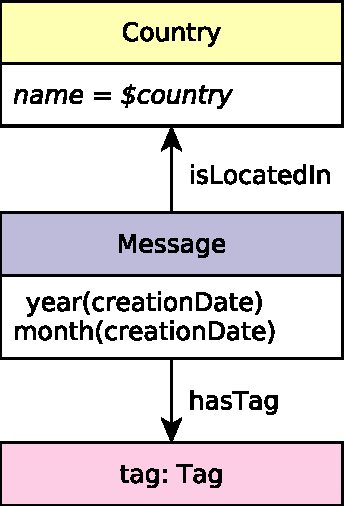
\includegraphics[scale=\patternscale,margin=0cm .2cm]{patterns/bi-read-13}\hfill\vadjust{} \\ \hline
%
	description & Find all Messages in a given Country, as well as their Tags.

For each group, find the 5 most popular Tags, where popularity is the
number of Messages (from within the same group) where the Tag appears.
 \\ \hline
%
	
	group by       &
	\multicolumn{1}{>{\raggedright}X|}{
		\varname{year}, 
		\varname{month}
		} \\ \hline
	
%
	parameters  &
	\vspace{1.1ex}{\begin{tabularx}{14.2cm}{|c|M|m{2cm}|Y|} \hline
	\cellcolor{black!70} \color{white} $\mathsf{1}$ & \varname{country} & \cellcolor{gray!20} \vartype{String} &  \\ \hline
	\end{tabularx}}\vspace{1.1ex} \\ \hline
%
	
	result      &
	\vspace{1.1ex}{\begin{tabularx}{14.2cm}{|c|M|m{2cm}|Y|} \hline
	\cellcolor{black!70} \color{white} $\mathsf{1}$ & \varname{year} & \cellcolor{gray!20} \vartype{32-bit Integer} & year(message.creationDate) \\ \hline
	\cellcolor{black!70} \color{white} $\mathsf{2}$ & \varname{month} & \cellcolor{gray!20} \vartype{32-bit Integer} & month(message.creationDate) \\ \hline
	\cellcolor{black!70} \color{white} $\mathsf{3}$ & \varname{popularTags} & \cellcolor{gray!20} \vartype{TagPairs} & (tag.name - String, popularity - 32-bit Integer), sorted descending by popularity, then ascending by tag name \\ \hline
	\end{tabularx}}\vspace{1.1ex} \\ \hline
	
%
	sort        &
	\vspace{1.1ex}{\begin{tabular}{|c|l|c|} \hline
	\cellcolor{black!70} \color{white} $\mathsf{1}$ & \varname{year} & \cellcolor{gray!20} $\desc$ \\ \hline
	\cellcolor{black!70} \color{white} $\mathsf{2}$ & \varname{month} & \cellcolor{gray!20} $\asc$ \\ \hline
	\end{tabular}}\vspace{1.1ex} \\ \hline
	%
	limit       & 100 \\ \hline
	%
	choke points &
	\multicolumn{1}{c}{  % >{\raggedright}x|}{
	  \chokepoint{1.2}, 
	  \chokepoint{2.2}, 
	  \chokepoint{2.3}, 
	  \chokepoint{3.2}, 
	  \chokepoint{6.1}
	  } \\ \hline
	%
\end{tabularx}
\renewcommand*{\arraystretch}{1.1}

\label{sec:bi-read-14}
\noindent\begin{tabularx}{\queryCardWidth}{|>{\queryPropertyCell}c|X|}
	\hline
	query & BI / 14 \\ \hline
%
	title & Top thread initiators \\ \hline
%
    pattern & \hfill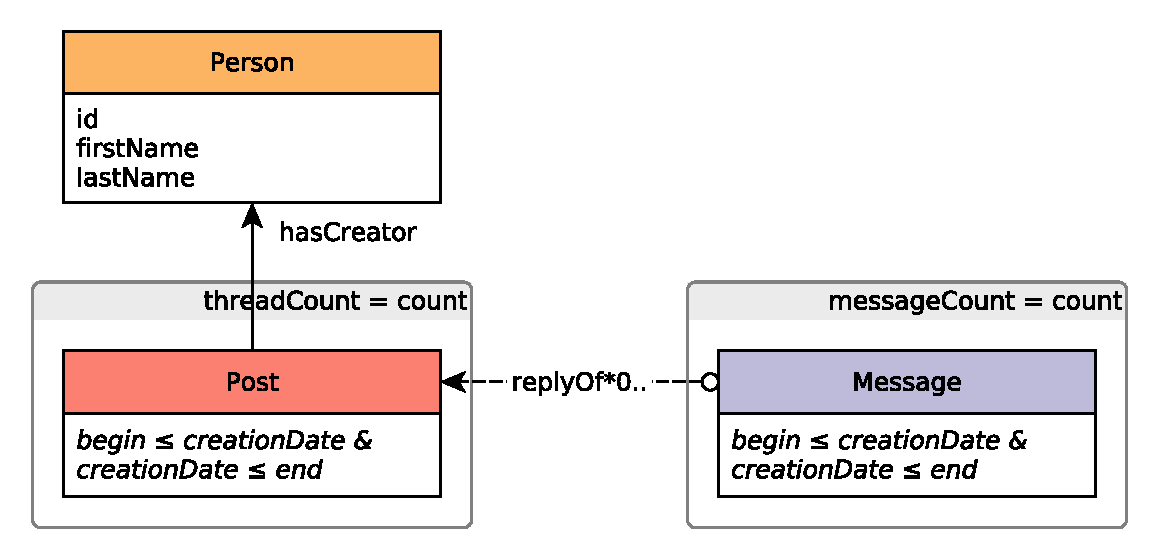
\includegraphics[scale=\patternscale,margin=0cm .2cm]{patterns/bi-read-14}\hfill\vadjust{} \\ \hline
%
	desc. & For each person, count the number Posts they created in the time
interval \texttt{(begin,\ end)}, and the number of messages in each of
their (transitive) reply trees. When calculating message counts only
consider messages created within the given time interval.

Return each person, number of Posts they created, and the count of all
messages that appeared in the reply trees (including Post at tree root)
they created.
 \\ \hline
%
	
%
	params &
	\innerCardVSpace{\begin{tabularx}{\attributeCardWidth}{|>{\paramNumberCell}c|>{\varNameCell}M|>{\typeCell}m{\typeWidth}|Y|} \hline
	\cellcolor{parameter} \color{white} \footnotesize $\mathsf{1}$ &begin& Date &  \\ \hline
	\cellcolor{parameter} \color{white} \footnotesize $\mathsf{2}$ &end& Date &  \\ \hline
	\end{tabularx}}\innerCardVSpace \\ \hline
%
	
        result &
        \innerCardVSpace{\begin{tabularx}{\attributeCardWidth}{|>{\resultNumberCell}c|>{\varNameCell}M|>{\typeCell}m{\typeWidth}|>{\resultOriginCell}c|Y|} \hline
        $\mathsf{1}$ & person.id & 64-bit Integer &R&
                 \\ \hline
        $\mathsf{2}$ & person.firstName & String &R&
                 \\ \hline
        $\mathsf{3}$ & person.lastName & String &R&
                 \\ \hline
        $\mathsf{4}$ & threadCount & 32-bit Integer &A&
                The number of threads initiated by that Person \\ \hline
        $\mathsf{5}$ & messageCount & 32-bit Integer &A&
                The number of messages created in all the threads this Person initiated \\ \hline
        \end{tabularx}}\innerCardVSpace \\ \hline
	
%
	sort        &
        \innerCardVSpace{\begin{tabular}{|>{\sortNumberCell}c|>{\varNameCell}l|>{\directionCell}c|} \hline
        $\mathsf{1}$ & messageCount & $\desc$ \\ \hline
        $\mathsf{2}$ & person.id & $\asc$ \\ \hline
        \end{tabular}}\innerCardVSpace \\ \hline
	%
	limit & 100 \\ \hline
	%
	CPs &
	\multicolumn{1}{>{\raggedright}l|}{
	    \chokePoint{1.2}, 
	    \chokePoint{2.2}, 
	    \chokePoint{2.3}, 
	    \chokePoint{3.2}, 
	    \chokePoint{7.2}, 
	    \chokePoint{7.3}, 
	    \chokePoint{7.4}
	    } \\ \hline
	%
    %
\end{tabularx}
\queryCardVSpace
\renewcommand*{\arraystretch}{1.1}

\subsection*{BI / read / 15}
\label{section:bi-read-15}

\noindent\begin{tabularx}{\queryCardWidth}{|>{\queryPropertyCell}p{\queryPropertyCellWidth}|X|}
	\hline
	query & BI / read / 15 \\ \hline
%
	title & Social normals
 \\ \hline
%
	pattern & \hfill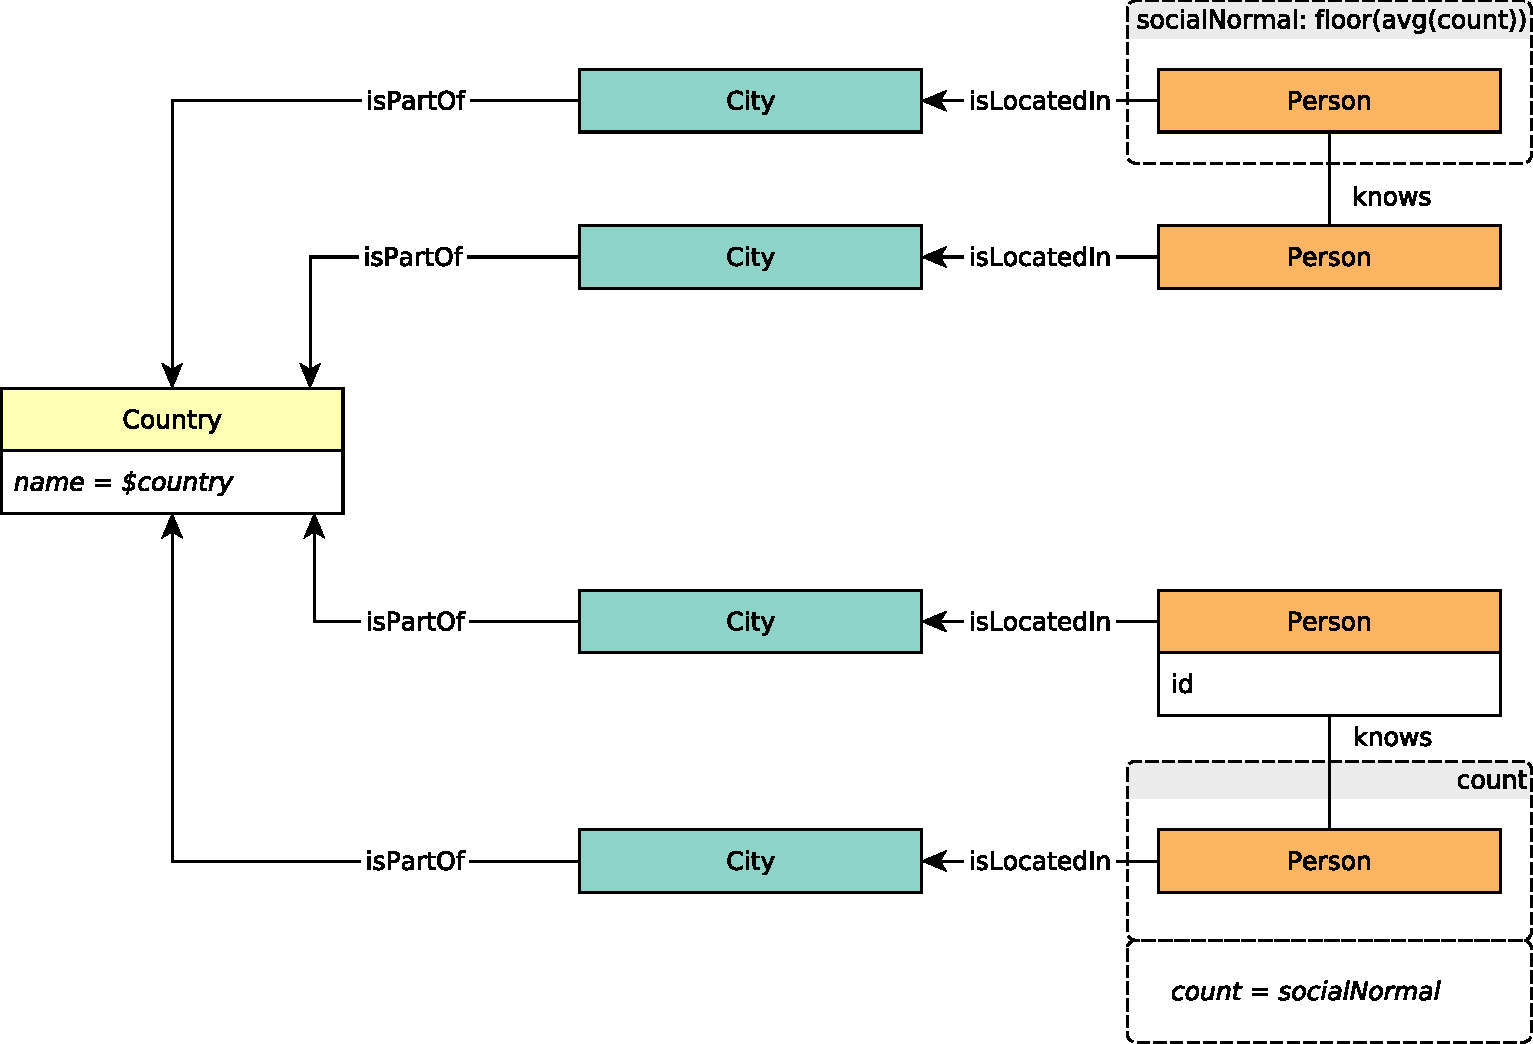
\includegraphics[scale=\patternscale,margin=0cm .2cm]{patterns/bi-read-15}\hfill\vadjust{} \\ \hline
%
	desc. & Given a \texttt{country}, find all \emph{Persons} of the \emph{Country}
whose number of friends in the given \emph{Country} equals the (floor
of) average number of friends that \emph{Persons} of the given
\emph{Country} have in the given \emph{country}.
 \\ \hline
%
	
		params &
		\innerCardVSpace{\begin{tabularx}{\attributeCardWidth}{|>{\paramNumberCell}c|>{\varNameCell}M|>{\typeCell}m{\typeWidth}|Y|} \hline
		$\mathsf{1}$ & country
 & 32-bit Integer
 &  \\ \hline
		\end{tabularx}}\innerCardVSpace \\ \hline
	
%
	
		result &
		\innerCardVSpace{\begin{tabularx}{\attributeCardWidth}{|>{\resultNumberCell}c|>{\varNameCell}M|>{\typeCell}m{\typeWidth}|>{\resultOriginCell}c|Y|} \hline
		$\mathsf{1}$ & person.id
 & 64-bit Integer
 & R &
				 \\ \hline
		$\mathsf{2}$ & count
 & 32-bit Integer
 & R &
				 \\ \hline
		\end{tabularx}}\innerCardVSpace \\ \hline
	
%
	
		sort		&
		\innerCardVSpace{\begin{tabularx}{\attributeCardWidth}{|>{\sortNumberCell}c|>{\varNameCell}M|>{\directionCell}c|Y|} \hline
		$\mathsf{1}$ & person.id
 & $\asc
$ &  \\ \hline
		\end{tabularx}}\innerCardVSpace \\ \hline
	%
	limit & 100 \\ \hline
	%
	CPs &
	\multicolumn{1}{>{\raggedright}l|}{
		\chokePoint{1.2}, 
		\chokePoint{2.3}, 
		\chokePoint{3.2}, 
		\chokePoint{3.3}, 
		\chokePoint{5.3}, 
		\chokePoint{6.1}
		} \\ \hline
	%
	%
\end{tabularx}
\queryCardVSpace
\renewcommand*{\arraystretch}{1.1}

\noindent\begin{tabularx}{17cm}{|p{1.95cm}|X|}
	\hline
	workload    & BI \\ \hline
%
	query       & 16 \\ \hline
%
	title       & Experts in social circle \\ \hline
%
    pattern     & \hfill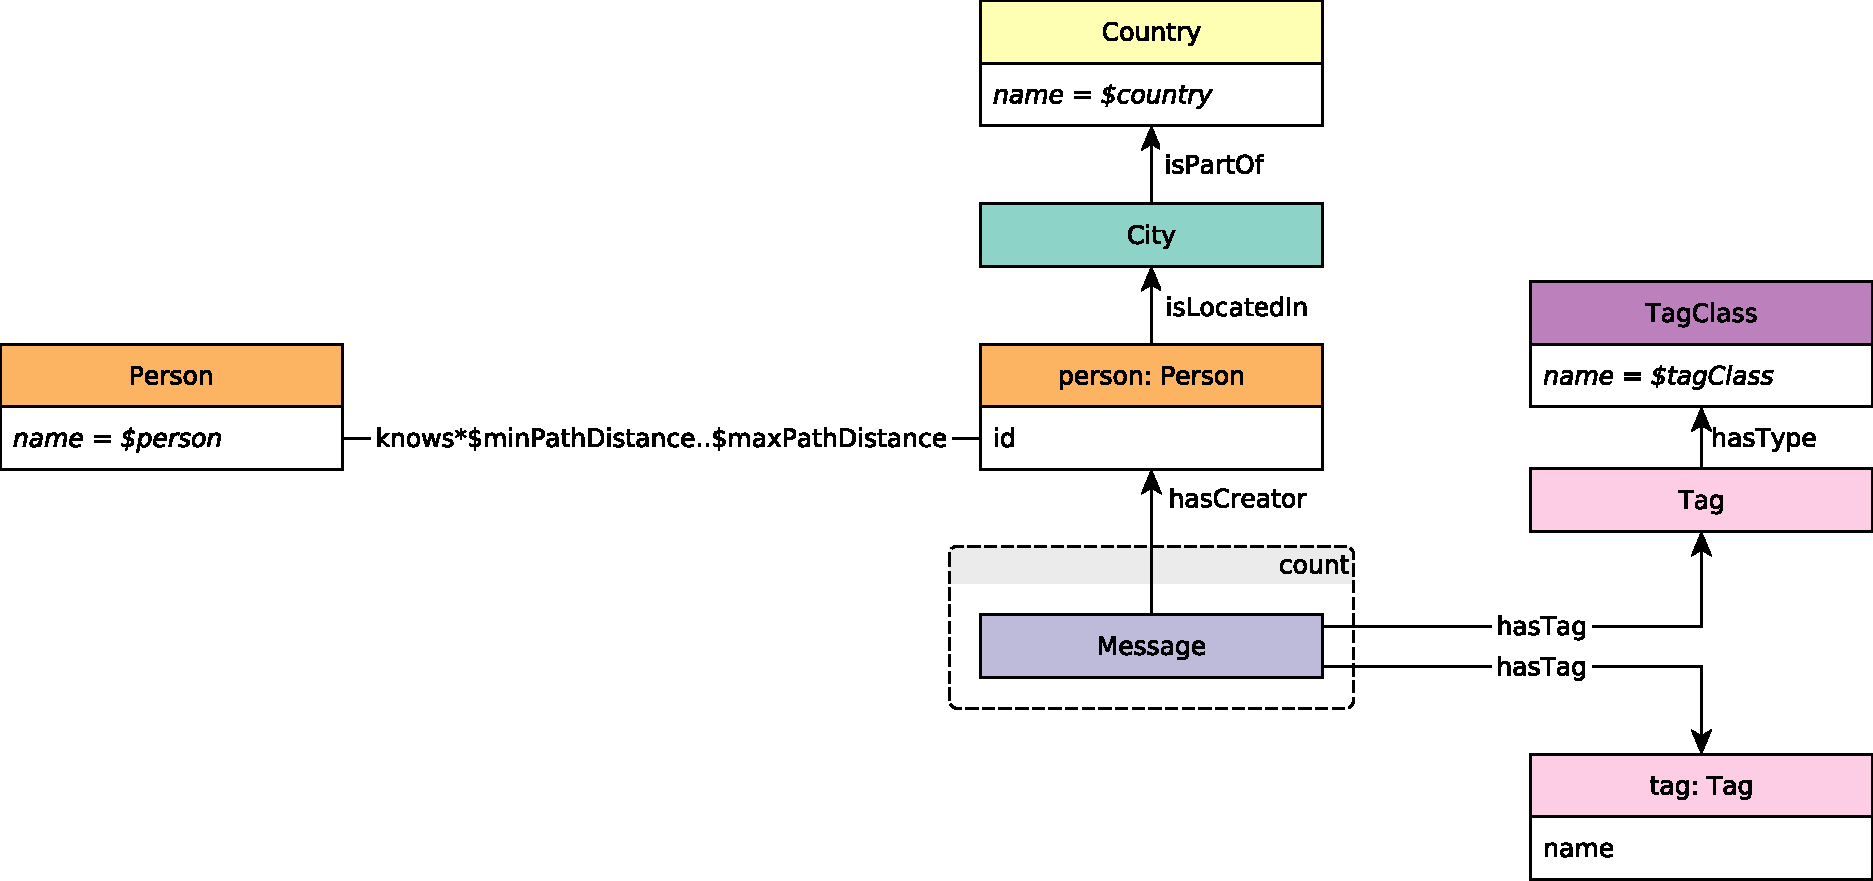
\includegraphics[scale=\patternscale,margin=0cm .2cm]{patterns/bi-read-16}\hfill\vadjust{} \\ \hline
%
	description & Given a Person, find all other Persons that live in a given country and
are connected to given person by a transitive path with length in range
\texttt{{[}min,\ max{]}} through the knows relation.

{[}DISCUSS: edge isomorphism semantics{]}

For each of these Persons, retrieve all of their Messages (Posts \&
Comments) that contain at least one Tag belonging to a given TagClass
(direct relation not transitive).

For each Message, also retrieve its Tags.

TODO {[}szarnyasg{]}: what is postCount?
 \\ \hline
%
	
	group by       &
	\multicolumn{1}{>{\raggedright}X|}{
		\varname{tag.name}, 
		\varname{person.id}
		} \\ \hline
	
%
	parameters  &
	\vspace{1.1ex}{\begin{tabularx}{14.2cm}{|c|M|m{2cm}|Y|} \hline
	\cellcolor{black!70} \color{white} $\mathsf{1}$ & \varname{personId} & \cellcolor{gray!20} \vartype{64-bit Integer} &  \\ \hline
	\cellcolor{black!70} \color{white} $\mathsf{2}$ & \varname{country} & \cellcolor{gray!20} \vartype{String} &  \\ \hline
	\cellcolor{black!70} \color{white} $\mathsf{3}$ & \varname{tagClass} & \cellcolor{gray!20} \vartype{String} &  \\ \hline
	\cellcolor{black!70} \color{white} $\mathsf{4}$ & \varname{minPathDistance} & \cellcolor{gray!20} \vartype{32-bit Integer} &  \\ \hline
	\cellcolor{black!70} \color{white} $\mathsf{5}$ & \varname{maxPathDistance} & \cellcolor{gray!20} \vartype{32-bit Integer} &  \\ \hline
	\end{tabularx}}\vspace{1.1ex} \\ \hline
%
	
	result      &
	\vspace{1.1ex}{\begin{tabularx}{14.2cm}{|c|M|m{2cm}|Y|} \hline
	\cellcolor{black!70} \color{white} $\mathsf{1}$ & \varname{person.id} & \cellcolor{gray!20} \vartype{64-bit Integer} &  \\ \hline
	\cellcolor{black!70} \color{white} $\mathsf{2}$ & \varname{tag.name} & \cellcolor{gray!20} \vartype{String} &  \\ \hline
	\cellcolor{black!70} \color{white} $\mathsf{3}$ & \varname{messageCount} & \cellcolor{gray!20} \vartype{32-bit Integer} & number of Messages created by that Person containing that Tag \\ \hline
	\end{tabularx}}\vspace{1.1ex} \\ \hline
	
%
	sort        &
	\vspace{1.1ex}{\begin{tabular}{|c|l|c|} \hline
	\cellcolor{black!70} \color{white} $\mathsf{1}$ & \varname{messageCount} & \cellcolor{gray!20} $\desc$ \\ \hline
	\cellcolor{black!70} \color{white} $\mathsf{2}$ & \varname{tag.name} & \cellcolor{gray!20} $\asc$ \\ \hline
	\cellcolor{black!70} \color{white} $\mathsf{3}$ & \varname{person.id} & \cellcolor{gray!20} $\asc$ \\ \hline
	\end{tabular}}\vspace{1.1ex} \\ \hline
	%
	limit       & 100 \\ \hline
	%
	choke points &
	\multicolumn{1}{c}{  % >{\raggedright}x|}{
	  \chokepoint{1.2}, 
	  \chokepoint{1.4}, 
	  \chokepoint{2.3}, 
	  \chokepoint{2.4}, 
	  \chokepoint{3.3}, 
	  \chokepoint{7.2}, 
	  \chokepoint{7.3}, 
	  \chokepoint{7.5}
	  } \\ \hline
	%
\end{tabularx}
\vspace{2ex}
\renewcommand*{\arraystretch}{1.1}

\subsection*{BI / read / 17}
\label{section:bi-read-17}

\noindent\begin{tabularx}{\queryCardWidth}{|>{\queryPropertyCell}p{\queryPropertyCellWidth}|X|}
	\hline
	query & BI / read / 17 \\ \hline
%
	title & Friend triangles
 \\ \hline
%
	pattern & \hfill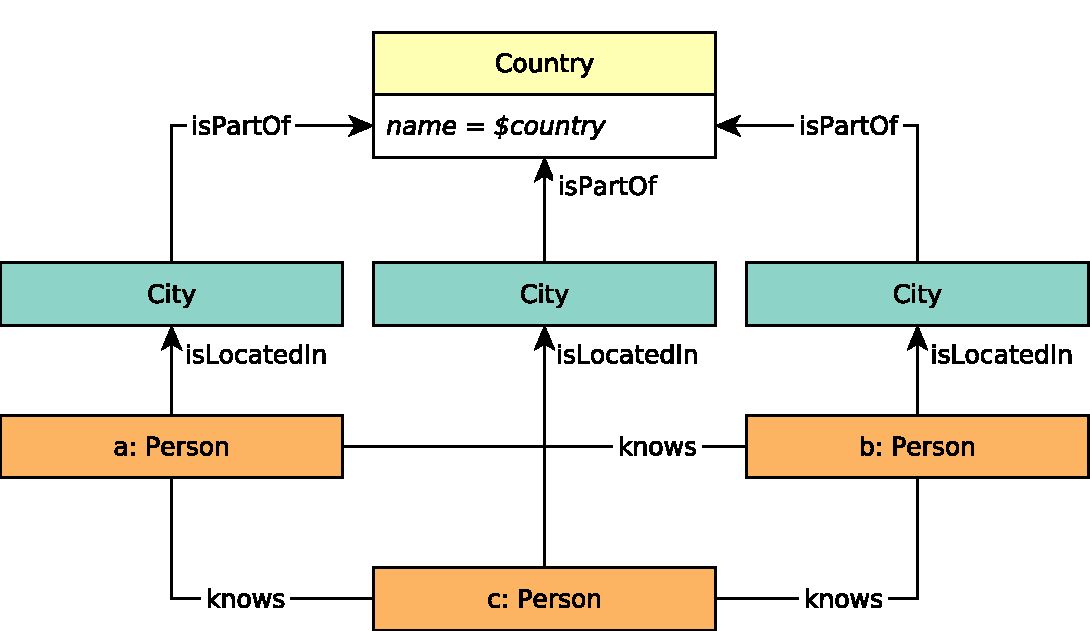
\includegraphics[scale=\patternscale,margin=0cm .2cm]{patterns/bi-read-17}\hfill\vadjust{} \\ \hline
%
	desc. & For a given \texttt{country}, count all the distinct triples of
\emph{Persons} such that \texttt{a} is friend of \texttt{b}, \texttt{b}
is friend of \texttt{c}, and \texttt{c} is friend of \texttt{a}.

Distinct means that given a triple \(t_1\) in the result set \(R\) of
all qualified triples, there is no triple \(t_2\) in \(R\) such that
\(t_1\) and \(t_2\) have the same set of elements.
 \\ \hline
%
	
		params &
		\innerCardVSpace{\begin{tabularx}{\attributeCardWidth}{|>{\paramNumberCell}c|>{\varNameCell}M|>{\typeCell}m{\typeWidth}|Y|} \hline
		$\mathsf{1}$ & country
 & String
 &  \\ \hline
		\end{tabularx}}\innerCardVSpace \\ \hline
	
%
	
		result &
		\innerCardVSpace{\begin{tabularx}{\attributeCardWidth}{|>{\resultNumberCell}c|>{\varNameCell}M|>{\typeCell}m{\typeWidth}|>{\resultOriginCell}c|Y|} \hline
		$\mathsf{1}$ & count & 32-bit Integer & A &
				 \\ \hline
		\end{tabularx}}\innerCardVSpace \\ \hline
	
%
	%
	%
	CPs &
	\multicolumn{1}{>{\raggedright}l|}{
		\chokePoint{1.1}, 
		\chokePoint{2.3}
		} \\ \hline
	%
	%
\end{tabularx}
\queryCardVSpace
\renewcommand*{\arraystretch}{1.1}

\subsection*{BI / read / 18}
\label{section:bi-read-18}

\noindent\begin{tabularx}{\queryCardWidth}{|>{\queryPropertyCell}p{\queryPropertyCellWidth}|X|}
	\hline
	query & BI / read / 18 \\ \hline
%
	title & How many persons have a given number of posts
 \\ \hline
%
	pattern & \hfill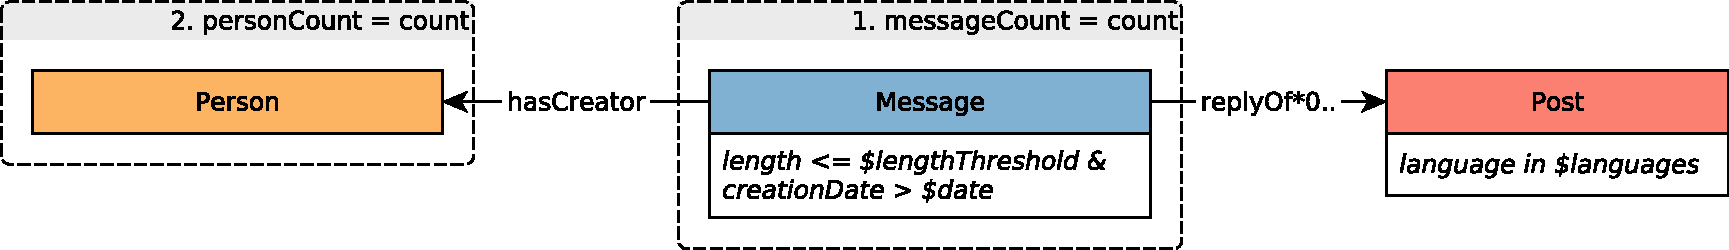
\includegraphics[scale=\patternscale,margin=0cm .2cm]{patterns/bi-read-18}\hfill\vadjust{} \\ \hline
%
	desc. & For each Person, count the number of Messages (Posts \& Comments) they
made.

Only consider messages with:

\begin{itemize}
\tightlist
\item
  length below the \texttt{lengthThreshold}
\item
  creationDate after \texttt{date} (exclusive, equality is not allowed)
\item
  any of the given \texttt{languages}
\end{itemize}

The language of a Comment is that of the Post that initiates the thread
where Comment belongs to.
 \\ \hline
%
	
		params &
		\innerCardVSpace{\begin{tabularx}{\attributeCardWidth}{|>{\paramNumberCell}c|>{\varNameCell}M|>{\typeCell}m{\typeWidth}|Y|} \hline
		$\mathsf{1}$ & date
 & Date
 &  \\ \hline
		$\mathsf{2}$ & lengthThreshold
 & 32-bit Integer
 &  \\ \hline
		$\mathsf{3}$ & languages
 & String{[}{]}
 &  \\ \hline
		\end{tabularx}}\innerCardVSpace \\ \hline
	
%
	
		result &
		\innerCardVSpace{\begin{tabularx}{\attributeCardWidth}{|>{\resultNumberCell}c|>{\varNameCell}M|>{\typeCell}m{\typeWidth}|>{\resultOriginCell}c|Y|} \hline
		$\mathsf{1}$ & messageCount
 & 32-bit Integer
 & R &
				Number of messages created
 \\ \hline
		$\mathsf{2}$ & personCount
 & 32-bit Integer
 & R &
				The number of Persons with \texttt{messageCount} messages
 \\ \hline
		\end{tabularx}}\innerCardVSpace \\ \hline
	
%
	
		sort		&
		\innerCardVSpace{\begin{tabular}{|>{\sortNumberCell}c|>{\varNameCell}l|>{\directionCell}c|} \hline
		$\mathsf{1}$ & personCount
 & $\desc
$ \\ \hline
		\end{tabular}}\innerCardVSpace \\ \hline
	%
	%
	CPs &
	\multicolumn{1}{>{\raggedright}l|}{
		\chokePoint{1.1}, 
		\chokePoint{1.2}, 
		\chokePoint{1.6}, 
		\chokePoint{3.2}, 
		\chokePoint{4.2}, 
		\chokePoint{4.3}
		} \\ \hline
	%
	%
\end{tabularx}
\queryCardVSpace
\renewcommand*{\arraystretch}{1.1}

\subsection*{BI / read / 19}
\label{section:bi-read-19}

% change \emph{} to use sans-serif font
\let\oldemph\emph
\renewcommand{\emph}[1]{{\footnotesize \sf #1}}

\renewcommand{\currentQueryCard}{19}
\marginpar{
	\raggedleft
	\vspace{0.22ex}

    \queryRefCard{bi-read-01}{BI}{1}\\
    \queryRefCard{bi-read-02}{BI}{2}\\
    \queryRefCard{bi-read-03}{BI}{3}\\
    \queryRefCard{bi-read-04}{BI}{4}\\
    \queryRefCard{bi-read-05}{BI}{5}\\
    \queryRefCard{bi-read-06}{BI}{6}\\
    \queryRefCard{bi-read-07}{BI}{7}\\
    \queryRefCard{bi-read-08}{BI}{8}\\
    \queryRefCard{bi-read-09}{BI}{9}\\
    \queryRefCard{bi-read-10}{BI}{10}\\
    \queryRefCard{bi-read-11}{BI}{11}\\
    \queryRefCard{bi-read-12}{BI}{12}\\
    \queryRefCard{bi-read-13}{BI}{13}\\
    \queryRefCard{bi-read-14}{BI}{14}\\
    \queryRefCard{bi-read-15}{BI}{15}\\
    \queryRefCard{bi-read-16}{BI}{16}\\
    \queryRefCard{bi-read-17}{BI}{17}\\
    \queryRefCard{bi-read-18}{BI}{18}\\
    \queryRefCard{bi-read-19}{BI}{19}\\
    \queryRefCard{bi-read-20}{BI}{20}\\
    \queryRefCard{bi-read-21}{BI}{21}\\
    \queryRefCard{bi-read-22}{BI}{22}\\
    \queryRefCard{bi-read-23}{BI}{23}\\
    \queryRefCard{bi-read-24}{BI}{24}\\
    \queryRefCard{bi-read-25}{BI}{25}\\
}


\noindent\begin{tabularx}{\queryCardWidth}{|>{\queryPropertyCell}p{\queryPropertyCellWidth}|X|}
	\hline
	query & BI / read / 19 \\ \hline
%
	title & Stranger's interaction
 \\ \hline
%
	pattern & \hfill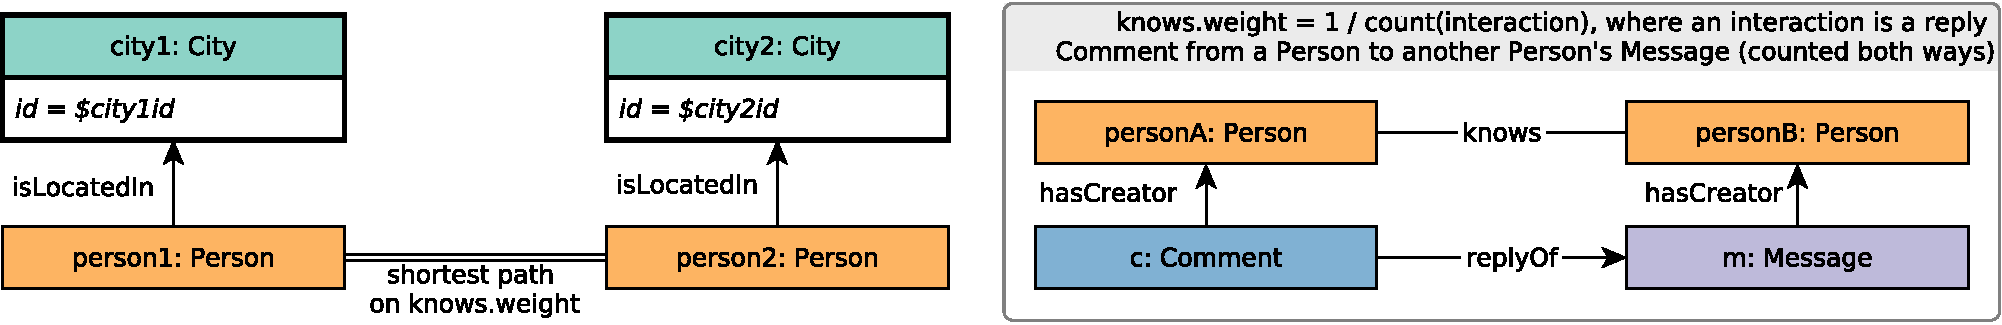
\includegraphics[scale=\patternscale,margin=0cm .2cm]{patterns/bi-read-19}\hfill\vadjust{} \\ \hline
%
	desc. & For all the \emph{Persons} born after a certain \texttt{date}, find all
the strangers they interacted with, where strangers are \emph{Persons}
that do not \emph{know} each other. There is no restriction on the date
that strangers were born.

Consider only strangers that are

\begin{itemize}
\tightlist
\item
  members of \emph{Forums} tagged with a \emph{Tag} with a (direct) type
  of \texttt{tagClass1} and
\item
  members of \emph{Forums} tagged with a \emph{Tag} with a (direct) type
  of \texttt{tagClass2}.
\end{itemize}

The tags may be attached to the same \emph{Forum} or they may be
attached to different \emph{Forums}.

Interaction is defined as follows: if \emph{Person} \emph{A} replies to
a \emph{Message} by another \emph{Person} \emph{B}, there is an
``interacted with'' relationship from \emph{A} to \emph{B}. Note that
the ``interacted with'' relationship is directed.

For each \emph{Person}, count the number of strangers they interacted
with and total number of times they interacted with them.
 \\ \hline
%
	
		params &
		\innerCardVSpace{\begin{tabularx}{\attributeCardWidth}{|>{\paramNumberCell}c|>{\varNameCell}M|>{\typeCell}m{\typeWidth}|Y|} \hline
		$\mathsf{1}$ & date
 & Date
 &  \\ \hline
		$\mathsf{2}$ & tagClass1
 & String
 &  \\ \hline
		$\mathsf{3}$ & tagClass2
 & String
 &  \\ \hline
		\end{tabularx}}\innerCardVSpace \\ \hline
	
%
	
		result &
		\innerCardVSpace{\begin{tabularx}{\attributeCardWidth}{|>{\resultNumberCell}c|>{\varNameCell}M|>{\typeCell}m{\typeWidth}|>{\resultOriginCell}c|Y|} \hline
		$\mathsf{1}$ & person.id & 64-bit Integer & R &
				 \\ \hline
		$\mathsf{2}$ & strangersCount & 32-bit Integer & A &
				 \\ \hline
		$\mathsf{3}$ & interactionCount & 32-bit Integer & A &
				 \\ \hline
		\end{tabularx}}\innerCardVSpace \\ \hline
	
%
	
		sort		&
		\innerCardVSpace{\begin{tabularx}{\attributeCardWidth}{|>{\sortNumberCell}c|>{\varNameCell}M|>{\directionCell}c|Y|} \hline
		$\mathsf{1}$ & interactionCount
 & $\desc
$ &  \\ \hline
		$\mathsf{2}$ & person.id
 & $\asc
$ &  \\ \hline
		\end{tabularx}}\innerCardVSpace \\ \hline
	%
	limit & 100 \\ \hline
	%
	CPs &
	\multicolumn{1}{>{\raggedright}l|}{
		\chokePoint{1.1}, 
		\chokePoint{1.4}, 
		\chokePoint{2.1}, 
		\chokePoint{2.3}, 
		\chokePoint{2.4}, 
		\chokePoint{3.3}, 
		\chokePoint{5.1}, 
		\chokePoint{7.3}, 
		\chokePoint{7.4}
		} \\ \hline
	%
	%
\end{tabularx}
\queryCardVSpace

% change \emph back to the old one
\renewcommand{\emph}[1]{\oldemph{#1}}
\renewcommand*{\arraystretch}{1.1}

\subsection*{BI / read / 20}
\label{section:bi-read-20}

% change \emph{} to use sans-serif font
\let\oldemph\emph
\renewcommand{\emph}[1]{{\footnotesize \sf #1}}

\renewcommand{\currentQueryCard}{20}
\marginpar{
	\raggedleft
	\vspace{0.22ex}

    \queryRefCard{bi-read-01}{BI}{1}\\
    \queryRefCard{bi-read-02}{BI}{2}\\
    \queryRefCard{bi-read-03}{BI}{3}\\
    \queryRefCard{bi-read-04}{BI}{4}\\
    \queryRefCard{bi-read-05}{BI}{5}\\
    \queryRefCard{bi-read-06}{BI}{6}\\
    \queryRefCard{bi-read-07}{BI}{7}\\
    \queryRefCard{bi-read-08}{BI}{8}\\
    \queryRefCard{bi-read-09}{BI}{9}\\
    \queryRefCard{bi-read-10}{BI}{10}\\
    \queryRefCard{bi-read-11}{BI}{11}\\
    \queryRefCard{bi-read-12}{BI}{12}\\
    \queryRefCard{bi-read-13}{BI}{13}\\
    \queryRefCard{bi-read-14}{BI}{14}\\
    \queryRefCard{bi-read-15}{BI}{15}\\
    \queryRefCard{bi-read-16}{BI}{16}\\
    \queryRefCard{bi-read-17}{BI}{17}\\
    \queryRefCard{bi-read-18}{BI}{18}\\
    \queryRefCard{bi-read-19}{BI}{19}\\
    \queryRefCard{bi-read-20}{BI}{20}\\
    \queryRefCard{bi-read-21}{BI}{21}\\
    \queryRefCard{bi-read-22}{BI}{22}\\
    \queryRefCard{bi-read-23}{BI}{23}\\
    \queryRefCard{bi-read-24}{BI}{24}\\
    \queryRefCard{bi-read-25}{BI}{25}\\
}



\noindent\begin{tabularx}{\queryCardWidth}{|>{\queryPropertyCell}p{\queryPropertyCellWidth}|X|}
	\hline
	query & BI / read / 20 \\ \hline
%
	title & High-level topics
 \\ \hline
%
	pattern & \hfill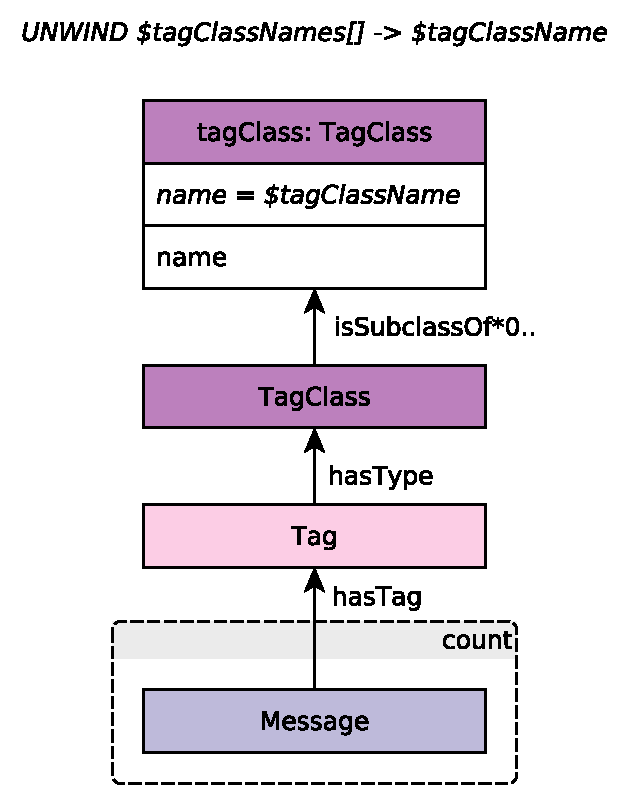
\includegraphics[scale=\patternscale,margin=0cm .2cm]{patterns/bi-read-20}\hfill\vadjust{} \\ \hline
%
	desc. & For all given \emph{TagClasses}, count number of \emph{Messages} that
have a \emph{Tag} that belongs to that \emph{TagClass} or any of its
children (all descendants through a transitive relation).
 \\ \hline
%
	
		params &
		\innerCardVSpace{\begin{tabularx}{\attributeCardWidth}{|>{\paramNumberCell}c|>{\varNameCell}M|>{\typeCell}m{\typeWidth}|Y|} \hline
		$\mathsf{1}$ & tagClasses
 & String{[}{]}
 &  \\ \hline
		\end{tabularx}}\innerCardVSpace \\ \hline
	
%
	
		result &
		\innerCardVSpace{\begin{tabularx}{\attributeCardWidth}{|>{\resultNumberCell}c|>{\varNameCell}M|>{\typeCell}m{\typeWidth}|>{\resultOriginCell}c|Y|} \hline
		$\mathsf{1}$ & tagClass.name & String & R &
				The \emph{TagClass} of the root
 \\ \hline
		$\mathsf{2}$ & postCount & 32-bit Integer & A &
				 \\ \hline
		\end{tabularx}}\innerCardVSpace \\ \hline
	
%
	
		sort		&
		\innerCardVSpace{\begin{tabularx}{\attributeCardWidth}{|>{\sortNumberCell}c|>{\varNameCell}M|>{\directionCell}c|Y|} \hline
		$\mathsf{1}$ & postCount
 & $\desc
$ &  \\ \hline
		$\mathsf{2}$ & tagClass.name
 & $\asc
$ &  \\ \hline
		\end{tabularx}}\innerCardVSpace \\ \hline
	%
	limit & 100 \\ \hline
	%
	CPs &
	\multicolumn{1}{>{\raggedright}l|}{
		\chokePoint{1.6}, 
		\chokePoint{2.1}, 
		\chokePoint{6.1}
		} \\ \hline
	%
	%
\end{tabularx}
\queryCardVSpace

% change \emph back to the old one
\renewcommand{\emph}[1]{\oldemph{#1}}
\renewcommand*{\arraystretch}{1.1}

\subsection*{BI / read / 21}
\label{section:bi-read-21}

% change \emph{} to use sans-serif font
\let\oldemph\emph
\renewcommand{\emph}[1]{{\footnotesize \sf #1}}

\renewcommand{\currentQueryCard}{21}
\marginpar{
	\raggedleft
	\vspace{0.22ex}

	\queryRefCard{bi-read-01}{BI}{1}\\
	\queryRefCard{bi-read-02}{BI}{2}\\
	\queryRefCard{bi-read-03}{BI}{3}\\
	\queryRefCard{bi-read-04}{BI}{4}\\
	\queryRefCard{bi-read-05}{BI}{5}\\
	\queryRefCard{bi-read-06}{BI}{6}\\
	\queryRefCard{bi-read-07}{BI}{7}\\
	\queryRefCard{bi-read-08}{BI}{8}\\
	\queryRefCard{bi-read-09}{BI}{9}\\
	\queryRefCard{bi-read-10}{BI}{10}\\
	\queryRefCard{bi-read-11}{BI}{11}\\
	\queryRefCard{bi-read-12}{BI}{12}\\
	\queryRefCard{bi-read-13}{BI}{13}\\
	\queryRefCard{bi-read-14}{BI}{14}\\
	\queryRefCard{bi-read-15}{BI}{15}\\
	\queryRefCard{bi-read-16}{BI}{16}\\
	\queryRefCard{bi-read-17}{BI}{17}\\
	\queryRefCard{bi-read-18}{BI}{18}\\
	\queryRefCard{bi-read-19}{BI}{19}\\
	\queryRefCard{bi-read-20}{BI}{20}\\
	\queryRefCard{bi-read-21}{BI}{21}\\
	\queryRefCard{bi-read-22}{BI}{22}\\
	\queryRefCard{bi-read-23}{BI}{23}\\
	\queryRefCard{bi-read-24}{BI}{24}\\
	\queryRefCard{bi-read-25}{BI}{25}\\
}


\noindent\begin{tabularx}{\queryCardWidth}{|>{\queryPropertyCell}p{\queryPropertyCellWidth}|X|}
	\hline
	query & BI / read / 21 \\ \hline
%
	title & Zombies in a country \\ \hline
%
	pattern & \hfill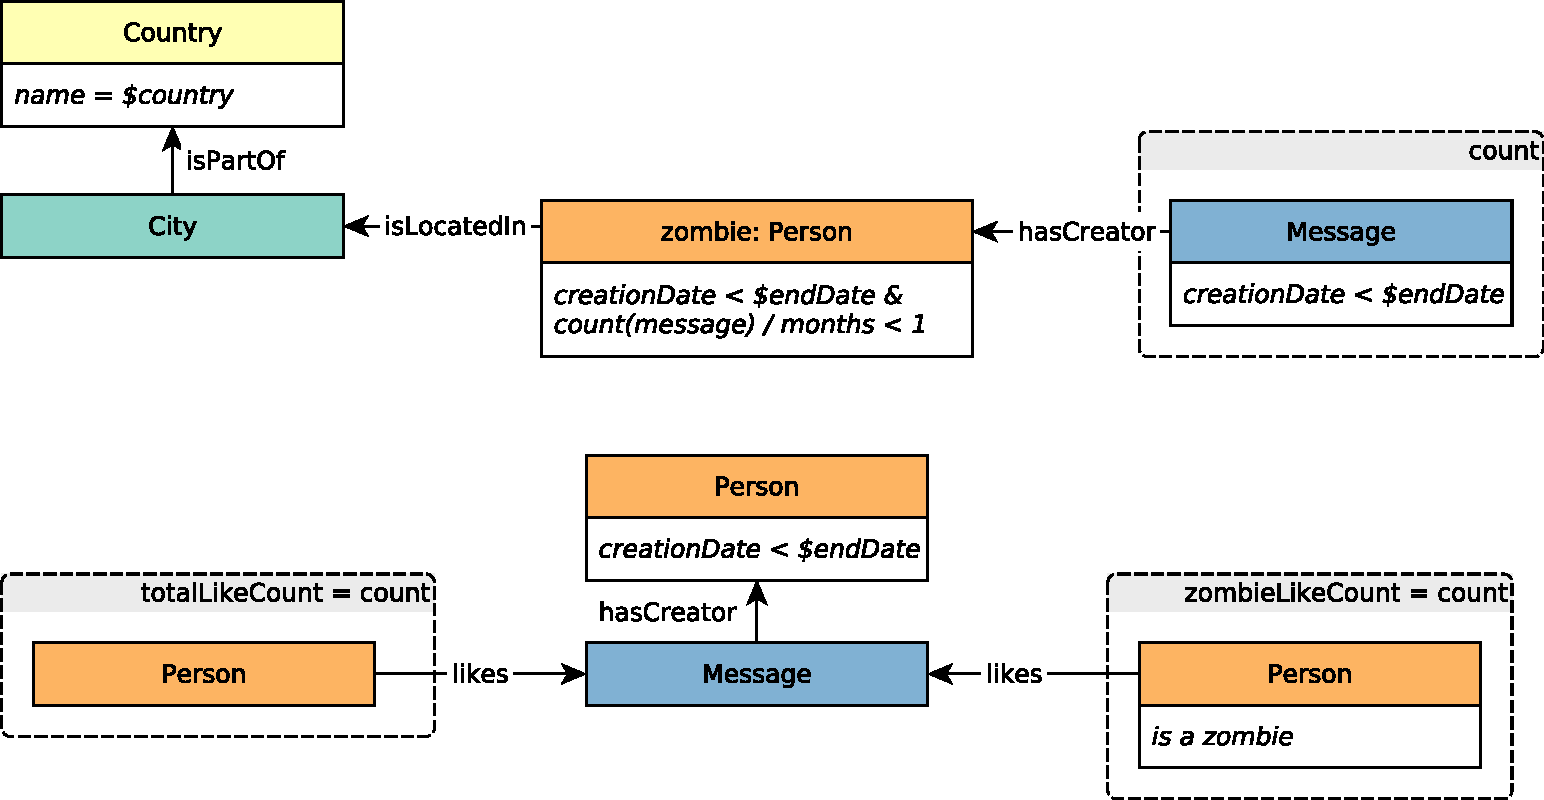
\includegraphics[scale=\patternscale,margin=0cm .2cm]{patterns/bi-read-21}\hfill\vadjust{} \\ \hline
%
	desc. & Find zombies within the given \texttt{country}, and return their zombie
scores. A \texttt{zombie} is a \emph{Person} created before the given
\texttt{endDate}, which has created an average of \texttt{{[}0,\ 1)}
\emph{Messages} per month, during the time range between profile's
\texttt{creationDate} and the given \texttt{endDate}. The number of
months spans the time range from the \texttt{creationDate} of the
profile to the \texttt{endDate} with partial months on both end counting
as one month (e.g.~a \texttt{creationDate} of Jan 31 and an
\texttt{endDate} of Mar 1 result in 3 months).

For each \texttt{zombie}, calculate the following:

\begin{itemize}
\tightlist
\item
  \texttt{zombieLikeCount}: the number of \emph{likes} received from
  other zombies.
\item
  \texttt{totalLikeCount}: the total number of \emph{likes} received.
\item
  \texttt{zombieScore}: \texttt{zombieLikeCount} /
  \texttt{totalLikeCount}. If the value of \texttt{totalLikeCount} is 0,
  the \texttt{zombieScore} of the \texttt{zombie} should be 0.
\end{itemize}

For both \texttt{zombieLikeCount} and \texttt{totalLikeCount}, only
consider \emph{likes} received from profiles that were created before
the given \texttt{endDate}.
 \\ \hline
%
	
		params &
		\innerCardVSpace{\begin{tabularx}{\attributeCardWidth}{|>{\paramNumberCell}c|>{\varNameCell}M|>{\typeCell}m{\typeWidth}|Y|} \hline
		$\mathsf{1}$ & country
 & String
 &  \\ \hline
		$\mathsf{2}$ & endDate
 & Date
 &  \\ \hline
		\end{tabularx}}\innerCardVSpace \\ \hline
	
%
	
		result &
		\innerCardVSpace{\begin{tabularx}{\attributeCardWidth}{|>{\resultNumberCell}c|>{\varNameCell}M|>{\typeCell}m{\typeWidth}|>{\resultOriginCell}c|Y|} \hline
		$\mathsf{1}$ & zombie.id & 64-bit Integer & R &
				 \\ \hline
		$\mathsf{2}$ & zombieLikeCount & 32-bit Integer & A &
				 \\ \hline
		$\mathsf{3}$ & totalLikeCount & 32-bit Integer & A &
				 \\ \hline
		$\mathsf{4}$ & zombieScore & 64-bit Float & A &
				\texttt{zombieLikeCount} / \texttt{totalLikeCount}
 \\ \hline
		\end{tabularx}}\innerCardVSpace \\ \hline
	
%
	
		sort		&
		\innerCardVSpace{\begin{tabularx}{\attributeCardWidth}{|>{\sortNumberCell}c|>{\varNameCell}M|>{\directionCell}c|Y|} \hline
		$\mathsf{1}$ & zombieScore
 & $\desc
$ &  \\ \hline
		$\mathsf{2}$ & zombie.id
 & $\asc
$ &  \\ \hline
		\end{tabularx}}\innerCardVSpace \\ \hline
	%
	limit & 100 \\ \hline
	%
	CPs &
	\multicolumn{1}{>{\raggedright}l|}{
		\chokePoint{1.2}, 
		\chokePoint{2.1}, 
		\chokePoint{2.3}, 
		\chokePoint{2.4}, 
		\chokePoint{3.2}, 
		\chokePoint{3.3}, 
		\chokePoint{5.1}, 
		\chokePoint{5.3}
		} \\ \hline
	%
	%
\end{tabularx}
\queryCardVSpace

% change \emph back to the old one
\renewcommand{\emph}[1]{\oldemph{#1}}
\renewcommand*{\arraystretch}{1.1}

\label{sec:bi-read-22}
\noindent\begin{tabularx}{\queryCardWidth}{|>{\queryPropertyCell}c|X|}
	\hline
	query & BI / read / 22 \\ \hline
%
	title & International dialog \\ \hline
%
    pattern & \hfill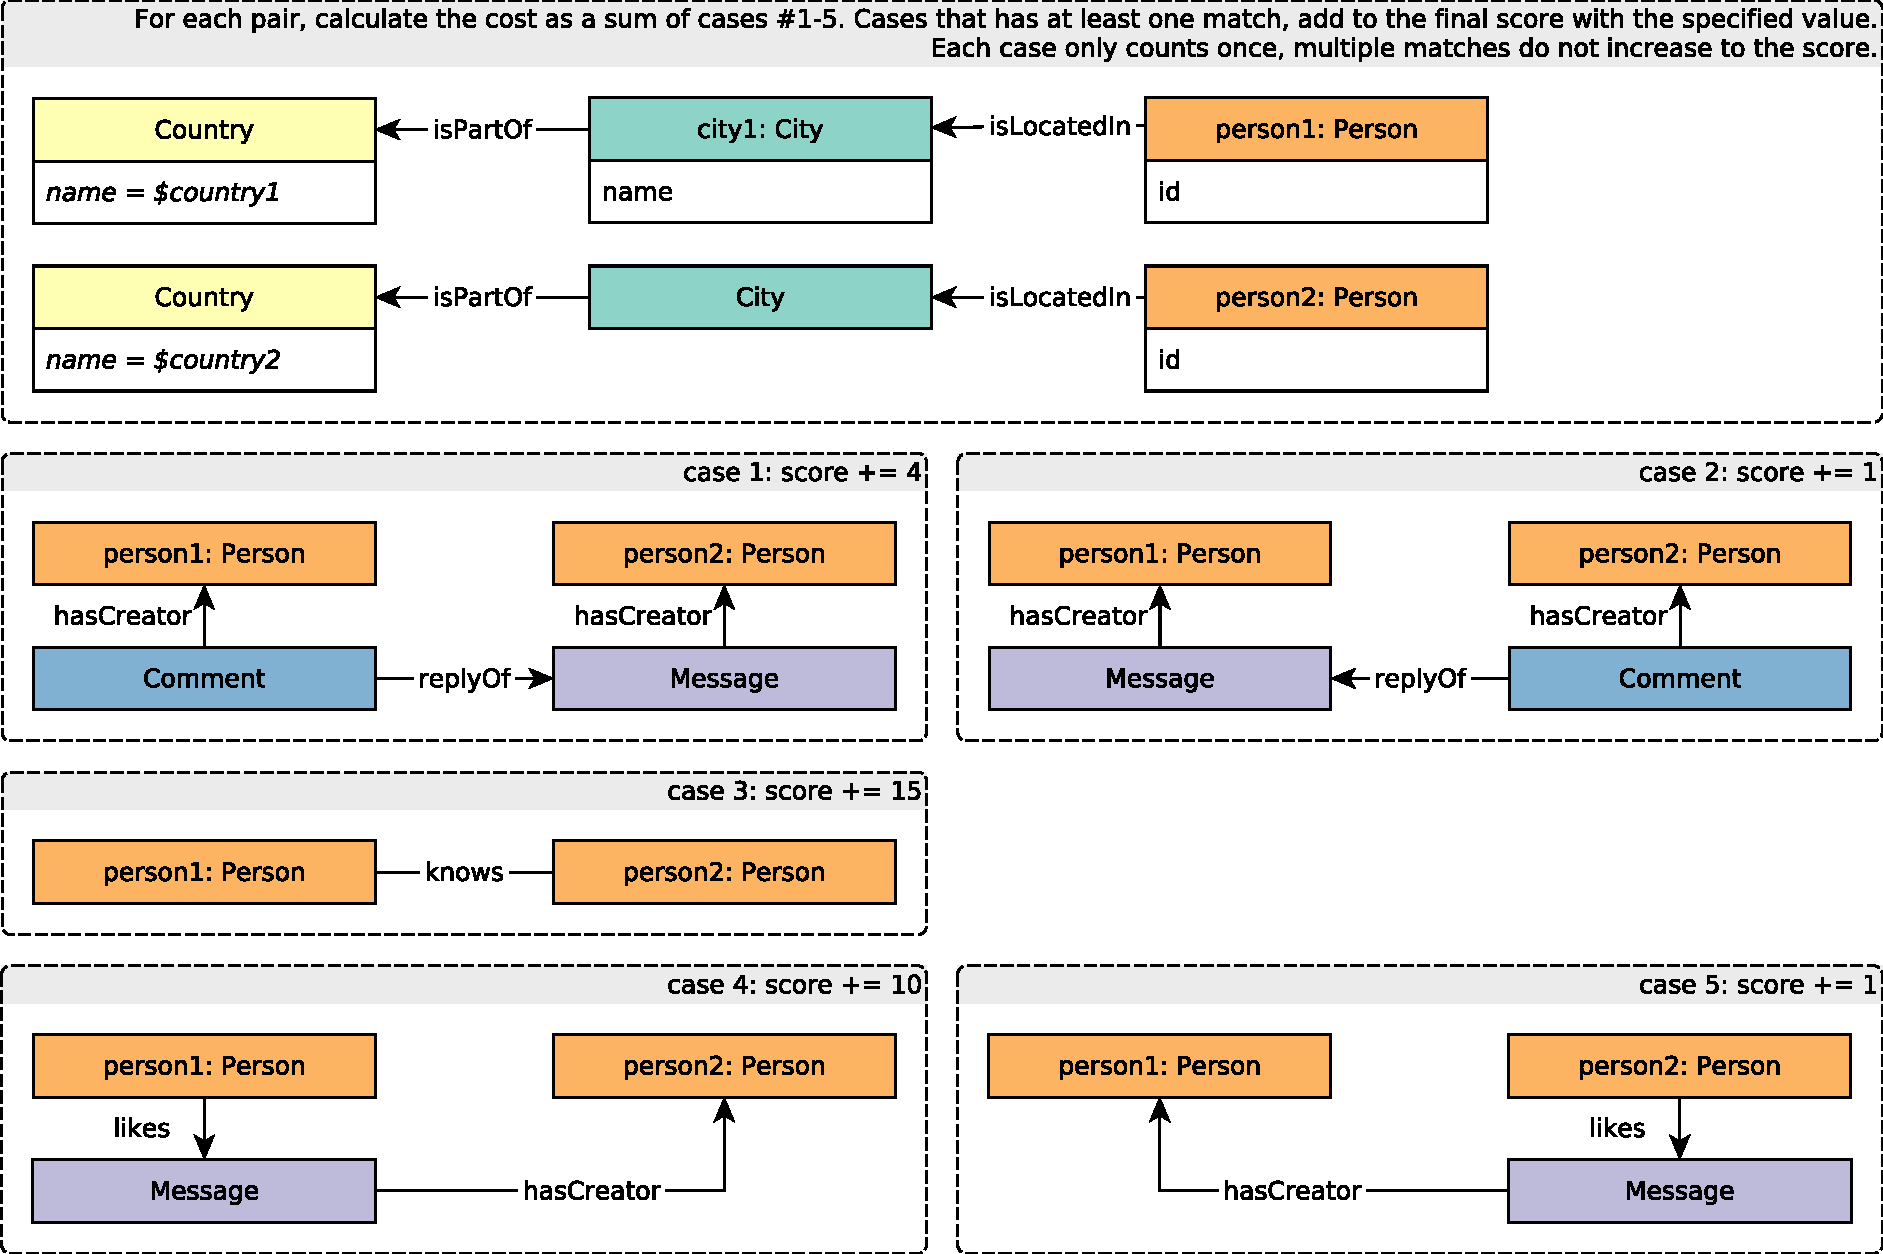
\includegraphics[scale=\patternscale,margin=0cm .2cm]{patterns/bi-read-22}\hfill\vadjust{} \\ \hline
%
	desc. & Consider all pairs of people \texttt{(p1,\ p2)} such that one is located
in a city of Country \texttt{countryX} and the other is located in a
city of Country \texttt{countryY}.

For each city of Country \texttt{countryX}, return the highest scoring
pair.

The score of a pair is defined as the sum of the scores of the following
kinds of interaction:

\begin{itemize}
\tightlist
\item
  \texttt{p1} has created a reply Comment to at least one Comment or
  Post by \texttt{p2}: \texttt{Score\ =\ 4}
\item
  \texttt{p1} has created at least one Post or Comment that \texttt{p2}
  has created a reply Comment to: \texttt{Score\ =\ 1}
\item
  \texttt{p1} and \texttt{p2} Know each other: \texttt{Score\ =\ 15}
\item
  \texttt{p1} liked at least one Post or Comment by \texttt{p2}:
  \texttt{Score\ =\ 10}
\item
  \texttt{p1} has created at least one Post or Comment that was liked by
  \texttt{p2}: \texttt{Score\ =\ 1}
\end{itemize}

I.e., the maximum score a pair can obtain is:
\texttt{4\ +\ 1\ +\ 15\ +\ 10\ +\ 1\ =\ 31}
 \\ \hline
%
	
%
    
        params &
        \innerCardVSpace{\begin{tabularx}{\attributeCardWidth}{|>{\paramNumberCell}c|>{\varNameCell}M|>{\typeCell}m{\typeWidth}|Y|} \hline
        \cellcolor{parameter} \color{white} \footnotesize $\mathsf{1}$ &countryX& String &  \\ \hline
        \cellcolor{parameter} \color{white} \footnotesize $\mathsf{2}$ &countryY& String &  \\ \hline
        \end{tabularx}}\innerCardVSpace \\ \hline
	
%
	
        result &
        \innerCardVSpace{\begin{tabularx}{\attributeCardWidth}{|>{\resultNumberCell}c|>{\varNameCell}M|>{\typeCell}m{\typeWidth}|>{\resultOriginCell}c|Y|} \hline
        $\mathsf{1}$ & p1.id & 64-bit Integer &R&
                 \\ \hline
        $\mathsf{2}$ & p2.id & 64-bit Integer &R&
                 \\ \hline
        $\mathsf{3}$ & cityX.name & String &R&
                 \\ \hline
        $\mathsf{4}$ & score & 32-bit Integer &C&
                 \\ \hline
        \end{tabularx}}\innerCardVSpace \\ \hline
	
%
	sort        &
        \innerCardVSpace{\begin{tabular}{|>{\sortNumberCell}c|>{\varNameCell}l|>{\directionCell}c|} \hline
        $\mathsf{1}$ & score & $\desc$ \\ \hline
        $\mathsf{2}$ & p1.id & $\asc$ \\ \hline
        $\mathsf{3}$ & p2.id & $\asc$ \\ \hline
        \end{tabular}}\innerCardVSpace \\ \hline
	%
	%
	CPs &
	\multicolumn{1}{>{\raggedright}l|}{
	    \chokePoint{1.4}, 
	    \chokePoint{1.6}, 
	    \chokePoint{2.1}, 
	    \chokePoint{3.1}, 
	    \chokePoint{3.3}, 
	    \chokePoint{5.1}, 
	    \chokePoint{5.2}, 
	    \chokePoint{5.3}
	    } \\ \hline
	%
    %
\end{tabularx}
\queryCardVSpace
\renewcommand*{\arraystretch}{1.1}

\subsection*{BI / read / 23}
\label{section:bi-read-23}

\noindent\begin{tabularx}{\queryCardWidth}{|>{\queryPropertyCell}p{\queryPropertyCellWidth}|X|}
	\hline
	query & BI / read / 23 \\ \hline
%
	title & Holiday destinations
 \\ \hline
%
	pattern & \hfill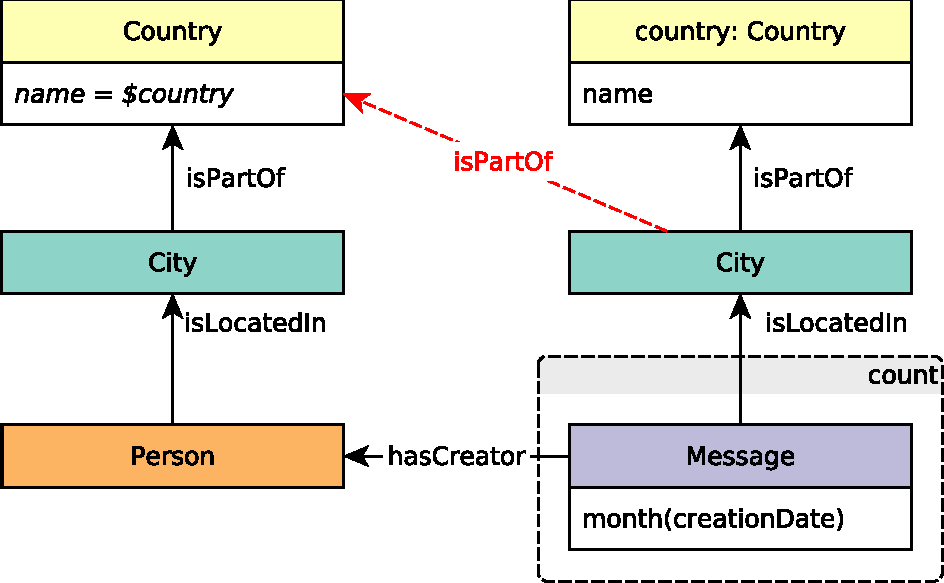
\includegraphics[scale=\patternscale,margin=0cm .2cm]{patterns/bi-read-23}\hfill\vadjust{} \\ \hline
%
	desc. & Count the \emph{Messages} all residents of a given \texttt{country} who
have written a \emph{Message} abroad, grouped by month and Country. A
\emph{Message} was written abroad if the \emph{Country} of the
\emph{Message} was written in is different than the \emph{Country} of
the \emph{Person} it was written by.
 \\ \hline
%
	
		params &
		\innerCardVSpace{\begin{tabularx}{\attributeCardWidth}{|>{\paramNumberCell}c|>{\varNameCell}M|>{\typeCell}m{\typeWidth}|Y|} \hline
		$\mathsf{1}$ & country
 & String
 &  \\ \hline
		\end{tabularx}}\innerCardVSpace \\ \hline
	
%
	
		result &
		\innerCardVSpace{\begin{tabularx}{\attributeCardWidth}{|>{\resultNumberCell}c|>{\varNameCell}M|>{\typeCell}m{\typeWidth}|>{\resultOriginCell}c|Y|} \hline
		$\mathsf{1}$ & messageCount & 32-bit Integer & A &
				The number of \emph{Messages} in each group
 \\ \hline
		$\mathsf{2}$ & country.name & String & R &
				The name of the destination \emph{Country}
 \\ \hline
		$\mathsf{3}$ & month & 32-bit Integer & C &
				 \\ \hline
		\end{tabularx}}\innerCardVSpace \\ \hline
	
%
	
		sort		&
		\innerCardVSpace{\begin{tabularx}{\attributeCardWidth}{|>{\sortNumberCell}c|>{\varNameCell}M|>{\directionCell}c|Y|} \hline
		$\mathsf{1}$ & messageCount
 & $\desc
$ &  \\ \hline
		$\mathsf{2}$ & country.name
 & $\asc
$ &  \\ \hline
		$\mathsf{3}$ & month
 & $\asc
$ &  \\ \hline
		\end{tabularx}}\innerCardVSpace \\ \hline
	%
	limit & 100 \\ \hline
	%
	CPs &
	\multicolumn{1}{>{\raggedright}l|}{
		\chokePoint{1.6}, 
		\chokePoint{2.3}, 
		\chokePoint{2.4}, 
		\chokePoint{3.3}, 
		\chokePoint{4.3}
		} \\ \hline
	%
	%
\end{tabularx}
\queryCardVSpace
\renewcommand*{\arraystretch}{1.1}

\noindent\begin{tabularx}{17cm}{|>{\small \sf}c|X|}
	\hline
	query    & BI / 24 \\ \hline
%
	title       & Messages by Topic and Continent \\ \hline
%
    pattern     & \hfill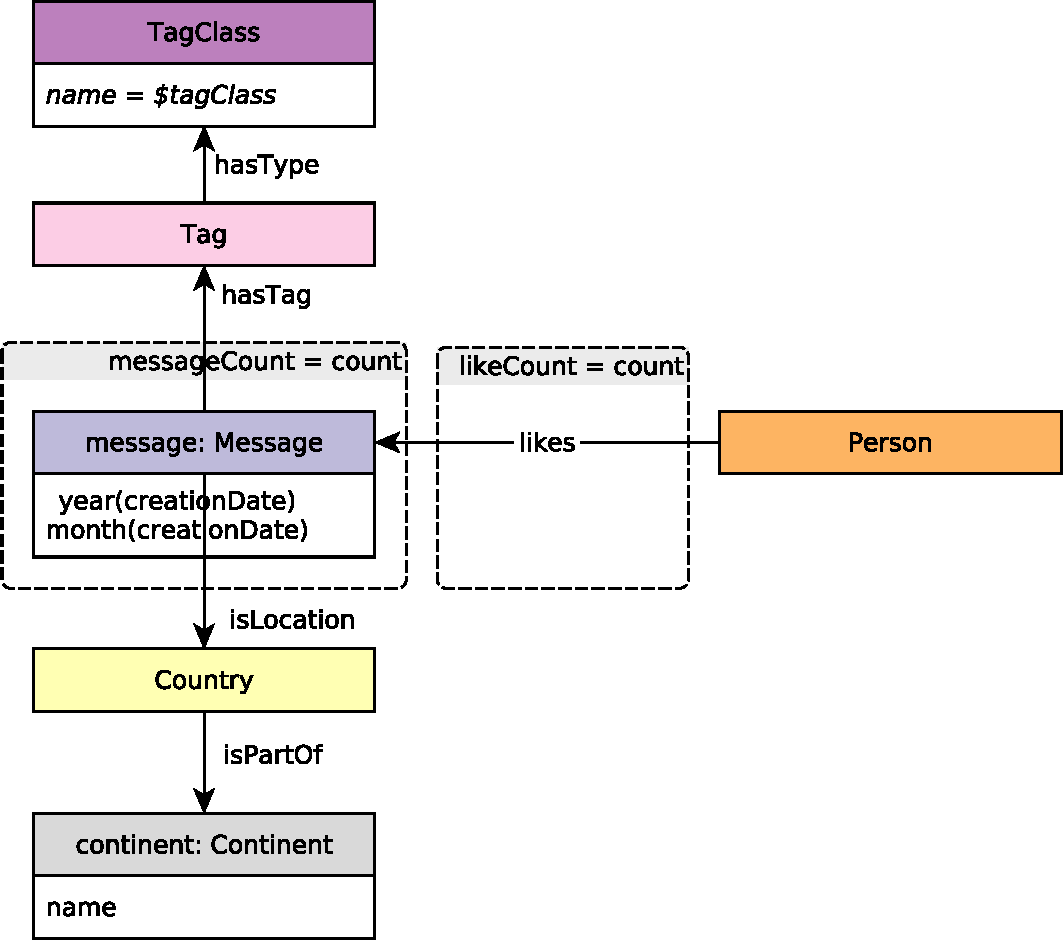
\includegraphics[scale=\patternscale,margin=0cm .2cm]{patterns/bi-read-24}\hfill\vadjust{} \\ \hline
%
	desc. & Find all Messages tagged with a Tag from the given TagClass
(non-transitive).

Count all messages and their likes grouped by continent, year, and
month. (TODO - do we group the Messages or the Persons who liked the
Messages by continent? I think the former one - szarnyasg)
 \\ \hline
%
	
	group by       &
	\multicolumn{1}{>{\raggedright}X|}{
		\varname{year}, 
		\varname{month}, 
		\varname{continent.name}
		} \\ \hline
	
%
	params.  &
	\vspace{1.1ex}{\begin{tabularx}{14.2cm}{|c|M|m{2cm}|Y|} \hline
	\cellcolor{parameter} \color{white} $\mathsf{1}$ & \varname{tagClass} & \cellcolor{gray!20} \vartype{String} &  \\ \hline
	\end{tabularx}}\vspace{1.1ex} \\ \hline
%
	
	result      &
	\vspace{1.1ex}{\begin{tabularx}{14.2cm}{|c|M|m{2cm}|c|Y|} \hline
	\cellcolor{result} \color{white} $\mathsf{1}$ & \varname{messageCount} & \cellcolor{gray!20} \vartype{32-bit Integer} &
	    \texttt{A} &
	     \\ \hline
	\cellcolor{result} \color{white} $\mathsf{2}$ & \varname{likeCount} & \cellcolor{gray!20} \vartype{32-bit Integer} &
	    \texttt{A} &
	     \\ \hline
	\cellcolor{result} \color{white} $\mathsf{3}$ & \varname{year} & \cellcolor{gray!20} \vartype{32-bit Integer} &
	    \texttt{C} &
	    year of the Message's creationDate \\ \hline
	\cellcolor{result} \color{white} $\mathsf{4}$ & \varname{month} & \cellcolor{gray!20} \vartype{32-bit Integer} &
	    \texttt{C} &
	    month of the Message's creationDate \\ \hline
	\cellcolor{result} \color{white} $\mathsf{5}$ & \varname{continent.name} & \cellcolor{gray!20} \vartype{String} &
	    \texttt{R} &
	     \\ \hline
	\end{tabularx}}\vspace{1.1ex} \\ \hline
	
%
	sort        &
	\vspace{1.1ex}{\begin{tabular}{|c|l|c|} \hline
	\cellcolor{sort} \color{white} $\mathsf{1}$ & \varname{year} & \cellcolor{gray!20} $\asc$ \\ \hline
	\cellcolor{sort} \color{white} $\mathsf{2}$ & \varname{month} & \cellcolor{gray!20} $\asc$ \\ \hline
	\cellcolor{sort} \color{white} $\mathsf{3}$ & \varname{continent.name} & \cellcolor{gray!20} $\desc$ \\ \hline
	\end{tabular}}\vspace{1.1ex} \\ \hline
	%
	limit       & 100 \\ \hline
	%
	CPs &
	\multicolumn{1}{>{\raggedright}l|}{
	  \chokepoint{1.6}, 
	  \chokepoint{2.1}, 
	  \chokepoint{2.3}, 
	  \chokepoint{2.4}, 
	  \chokepoint{3.2}, 
	  \chokepoint{4.3}
	  } \\ \hline
	%
    %
\end{tabularx}
\vspace{2ex}
\renewcommand*{\arraystretch}{1.1}

\subsection*{BI / read / 25}
\label{section:bi-read-25}

% change \emph{} to use sans-serif font
\let\oldemph\emph
\renewcommand{\emph}[1]{{\footnotesize \sf #1}}

\renewcommand{\currentQueryCard}{25}
\marginpar{
	\raggedleft
	\vspace{0.22ex}

	\queryRefCard{bi-read-01}{BI}{1}\\
	\queryRefCard{bi-read-02}{BI}{2}\\
	\queryRefCard{bi-read-03}{BI}{3}\\
	\queryRefCard{bi-read-04}{BI}{4}\\
	\queryRefCard{bi-read-05}{BI}{5}\\
	\queryRefCard{bi-read-06}{BI}{6}\\
	\queryRefCard{bi-read-07}{BI}{7}\\
	\queryRefCard{bi-read-08}{BI}{8}\\
	\queryRefCard{bi-read-09}{BI}{9}\\
	\queryRefCard{bi-read-10}{BI}{10}\\
	\queryRefCard{bi-read-11}{BI}{11}\\
	\queryRefCard{bi-read-12}{BI}{12}\\
	\queryRefCard{bi-read-13}{BI}{13}\\
	\queryRefCard{bi-read-14}{BI}{14}\\
	\queryRefCard{bi-read-15}{BI}{15}\\
	\queryRefCard{bi-read-16}{BI}{16}\\
	\queryRefCard{bi-read-17}{BI}{17}\\
	\queryRefCard{bi-read-18}{BI}{18}\\
	\queryRefCard{bi-read-19}{BI}{19}\\
	\queryRefCard{bi-read-20}{BI}{20}\\
	\queryRefCard{bi-read-21}{BI}{21}\\
	\queryRefCard{bi-read-22}{BI}{22}\\
	\queryRefCard{bi-read-23}{BI}{23}\\
	\queryRefCard{bi-read-24}{BI}{24}\\
	\queryRefCard{bi-read-25}{BI}{25}\\
}


\noindent\begin{tabularx}{\queryCardWidth}{|>{\queryPropertyCell}p{\queryPropertyCellWidth}|X|}
	\hline
	query & BI / read / 25 \\ \hline
%
	title & Weighted interaction paths
 \\ \hline
%
	pattern & \hfill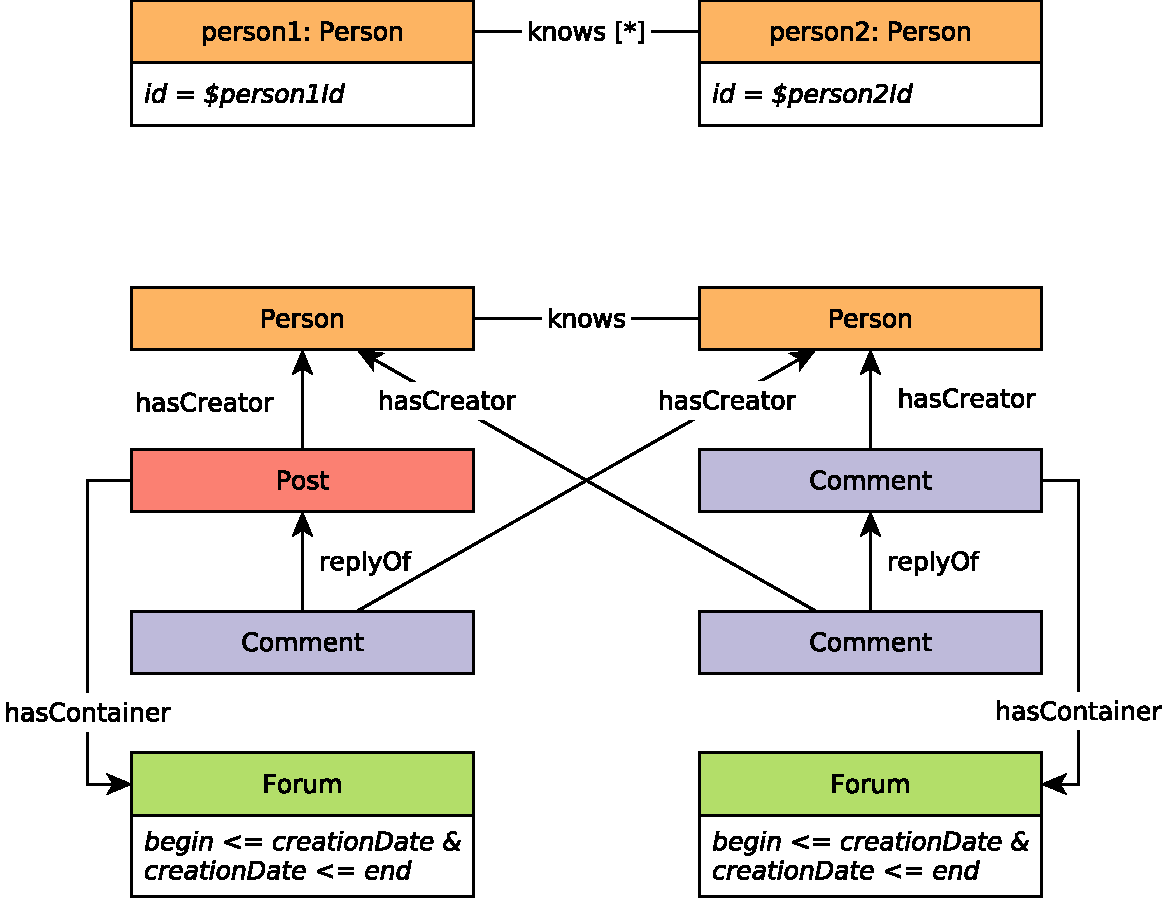
\includegraphics[scale=\patternscale,margin=0cm .2cm]{patterns/bi-read-25}\hfill\vadjust{} \\ \hline
%
	desc. & Given two \emph{Persons}, find all (unweighted) shortest paths between
these two \emph{Persons}, in the subgraph induced by the \emph{knows}
relationship.

Then, for each path calculate a weight. The nodes in the path are
\emph{Persons}, and the weight of a path is the sum of weights between
every pair of consecutive \emph{Person} nodes in the path.

The weight for a pair of \emph{Persons} is calculated based on their
interactions:

\begin{itemize}
\tightlist
\item
  Every reply (by one of the \emph{Persons}) to a \emph{Post} (by the
  other \emph{Person}) contributes 1.0.
\item
  Every reply (by one of the \emph{Persons}) to a \emph{Comment} (by the
  other \emph{Person}) contributes 0.5.
\end{itemize}

Only consider \emph{Messages} that were created in a \emph{Forum} that
was created within the timeframe \texttt{{[}startDate,\ endDate{]}}.

Return all the paths with shortest length, and their weights.
 \\ \hline
%
	
		params &
		\innerCardVSpace{\begin{tabularx}{\attributeCardWidth}{|>{\paramNumberCell}c|>{\varNameCell}M|>{\typeCell}m{\typeWidth}|Y|} \hline
		$\mathsf{1}$ & person1Id
 & 64-bit Integer
 &  \\ \hline
		$\mathsf{2}$ & person2Id
 & 64-bit Integer
 &  \\ \hline
		$\mathsf{3}$ & startDate
 & Date
 &  \\ \hline
		$\mathsf{4}$ & endDate
 & Date
 &  \\ \hline
		\end{tabularx}}\innerCardVSpace \\ \hline
	
%
	
		result &
		\innerCardVSpace{\begin{tabularx}{\attributeCardWidth}{|>{\resultNumberCell}c|>{\varNameCell}M|>{\typeCell}m{\typeWidth}|>{\resultOriginCell}c|Y|} \hline
		$\mathsf{1}$ & person.id & 64-bit Integer{[}{]} & R &
				Identifiers representing an ordered sequence of the \emph{Persons} in
the path weight
 \\ \hline
		\end{tabularx}}\innerCardVSpace \\ \hline
	
%
	
		sort		&
		\innerCardVSpace{\begin{tabularx}{\attributeCardWidth}{|>{\sortNumberCell}c|>{\varNameCell}M|>{\directionCell}c|Y|} \hline
		$\mathsf{1}$ & weight
 & $\desc
$ & The order of paths with the same weight is unspecified
 \\ \hline
		\end{tabularx}}\innerCardVSpace \\ \hline
	%
	%
	CPs &
	\multicolumn{1}{>{\raggedright}l|}{
		\chokePoint{1.2}, 
		\chokePoint{2.1}, 
		\chokePoint{2.2}, 
		\chokePoint{2.4}, 
		\chokePoint{3.3}, 
		\chokePoint{5.1}, 
		\chokePoint{5.3}, 
		\chokePoint{7.2}, 
		\chokePoint{7.3}
		} \\ \hline
	%
	%
\end{tabularx}
\queryCardVSpace

% change \emph back to the old one
\renewcommand{\emph}[1]{\oldemph{#1}}

% reset counter to make sure the last query card isn't stuck in highlighted mode
\renewcommand{\currentQueryCard}{0}


%%%%%%%%%%%%%%%%%%%%%%%%%%%%%%%%%%%%%%%%%%%%%%%%%%%%%%%%%%%%%%%%%%%%%%%%%%%%%%
%%%%%%%%%%%%%%%%%%%%%%%%%%%%%%%%%%%%%%%%%%%%%%%%%%%%%%%%%%%%%%%%%%%%%%%%%%%%%%
%%%%%%%%%%%%%%%%%%%%%%%%%%%%%%%%%%%%%%%%%%%%%%%%%%%%%%%%%%%%%%%%%%%%%%%%%%%%%%

\section{Insert Operations}
\label{sec:bi-insert-operations}

Insert operations consist of individual inserts for each entity type.
Implementations typically use the same format as the one for loading the initial snapshot of the data set.

%%%%%%%%%%%%%%%%%%%%%%%%%%%%%%%%%%%%%%%%%%%%%%%%%%%%%%%%%%%%%%%%%%%%%%%%%%%%%%
%%%%%%%%%%%%%%%%%%%%%%%%%%%%%%%%%%%%%%%%%%%%%%%%%%%%%%%%%%%%%%%%%%%%%%%%%%%%%%
%%%%%%%%%%%%%%%%%%%%%%%%%%%%%%%%%%%%%%%%%%%%%%%%%%%%%%%%%%%%%%%%%%%%%%%%%%%%%%

\section{Delete Operations}
\label{sec:bi-delete-operations}
\iftoggle{StandaloneWorkloadSpecification}{
    \input{query-cards/delete-01}
\input{query-cards/delete-02}
\input{query-cards/delete-03}
\input{query-cards/delete-04}
\input{query-cards/delete-05}
\input{query-cards/delete-06}
\input{query-cards/delete-07}
\input{query-cards/delete-08}

}{
    See \autoref{sec:delete-operations}.
}
